\documentclass{include/tfgitic}[2022/06/30]

%\usepackage{}

\addbibresource{misc/tfg.bib}

\title{Implementació d'una pantalla inte\l.ligent}
\subtitle{Creació d'un dispositiu i programari que actualitzi l'orientació
          d'una pantalla al rotar-la}

\author{Eric Roy Almonacid}
\advisor{Francisco del Águila López}

\dedication{Per l'avi, que hagués sigut el primer comprador d'aquest producte}

\begin{acknowledgments}
    Aquest treball no hagués existit si no fos per l'Isaac Iglesias, que em va
    proposar fer aquest projecte, i a poc a poc ha vist com la seva idea anava
    convertint-se en un producte.

    Una altra persona a qui dec aquest treball és al meu tutor del projecte, el
    Francisco del Águila, que m'ha orientat i recolzat durant tot aquest procés.

    També voldria agrair al professorat de l'EPSEM, però en especial al Joan
    Martínez que, juntamtent amb el meu tutor, m'ha aconsellat durant el disseny
    de la placa de circuit imprès.

    L'absència de faltes lingüístiques en aquest document és un mèrit de la
    meva parella, l'Aida Vers, que ha realitzat una correcció exhaustiva del
    treabll.

    Finalment, vull donar les gràcies a totes les persones del meu entorn
    quotidià que, potser fins i tot sense ells saber-ho, han fet que aquests
    mesos no semblin tan durs. Familiars, amics, companys de feina i d'estudis,
    aquest treball també és vostre.
\end{acknowledgments}

\begin{resum}
    La tendència a generar contingut audiovisual en format vertical és una de
    les diverses causes per la qual la gent es plantegi tenir una pantalla de
    l'ordinador en aquesta nova orientació. 
    Una de les solucions més senzilles i econòmiques és adquirir un suport de
    monitor que permeti rotar la pantalla sense haver-la de desmuntar, i així
    disposar fàcilment de les dues orientacions.

    Un inconvenient d'aquest sistema és que, quan es gira la pantalla, s'ha de
    reconfigurar l'entorn gràfic per adaptar-lo a la nova orientació.
    Existeixen alguns monitors d'alta gamma que, mitjançant la connexió d'imatge
    ja existent, poden notificar l'ordinador els canvis d'orientació. Tanmateix,
    aquests sistemes només funcionen correctament si s'utilitza el suport de
    pantalla i protocols recomanats.

    Aquest projecte proposa un dispositiu de baix cost que, mitjançant un sensor
    giroscòpic i una connexió USB, detecta l'orientació de la pantalla i
    configura l'entorn gràfic adequadament. S'ha posat èmfasi en l'ús de
    protocols estàndards existents, la compatibilitat entre diferents sistemes
    operatius i la facilitat d'insta\l.lació i ús dels programes relacionats
    amb el dispositiu.
\end{resum}

\begin{abstract}
    The trend towards generating audiovisual content in vertical format is one
    of the various reasons why people consider having a computer screen in this
    new orientation.
    One of the simplest and most economical solutions is to acquire a monitor
    stand that allows the screen to be rotated without having to disassemble it,
    thus easily providing both orientations.

    One drawback of this system is that when the screen is rotated, the graphic
    environment needs to be reconfigured to adapt to the new orientation.
    There are some high-end monitors that, through the existing image
    connection, can notify the computer of orientation changes. However,
    these systems only work properly if the recommended screen support and
    protocols are used.

    This project proposes a low-cost device that, using a gyroscope sensor and a
    USB connection, detects the screen orientation and configures the graphic
    environment accordingly. Emphasis has been placed on the use of existing
    standard protocols, compatibility between different operating systems, and
    the ease of installation and use of device-related programs.
\end{abstract}

\begin{document}

%\part{Memòria}

\chapter{Introducció}
\label{cap:introduccio}

Durant els darrers anys, el contingut digital en format vertical no ha cessat
d'augmentar, sent una de les principals causes l'ús generalitzat dels
dispositius mòbils \cite{Navarro2023El}. Les xarxes socials no van tardar a
adaptar les seves interfícies a aquestes noves resolucions. De fet, aquesta
tendència també s'ha portat a moltes altres aplicacions, tan de mòbil com
d'escriptori. Per exemple, han nascut termes com el
\est{Mobile-First Web Design}, que incita als desenvolupadors de pàgines web
a dissenyar les pàgines per a dispositius mòbils, i adaptar-les després
(el contrari del que es feia tradicionalment) \cite{varrela2015mobile}.

Tot plegat ha creat una nova moda: tenir una pantalla en vertical
en un ordinador de sobretaula. La majoria de monitors es poden muntar en
aquesta orientació sense necessitar un altre suport, pel que aquesta pràctica
s'ha popularitzat molt fàcilment \cite{WeardenPortrait}.
Disposar d'una pentalla en vertical també pot aportar altres avantatges. Per
exemple: els desenvolupadors poden veure més línies d'un mateix fitxer de codi
a la vegada, els dissenyadors de cartells o continguts per a dispositius mòbils
també poden beneficiar-se d'aquesta orientació.

Tanmateix, de vegades pot resultar més útil veure contingut en format
horizontal, com per exemple les pe\l.lícules. Si disposem de la configuració
anterior, hauríem de desmuntar la pantalla del suport i tornar-la a co\l.locar
en l'orientació desitjada. Un cop fet això, s'hauria d'anar a la configuració
del sistema per a que l'entorn gràfic del sistema operatiu mostri els continguts
d'aquella pantalla correctament. Aquest cúmul de tasques fan aquest procediment
tediós, sent aquest un motiu pel que no es sol dur a terme.

Per a resoldre aquest problema, han sortit a la venda suports rotatoris per a 
monitors \cite{DIGITUSUniversal}. Aquests redueixen el problema mencionat
anteriorment a només haver de girar la pantalla amb la força de la mà, i
configurar l'entorn gràfic. Algunes marques han anat més enllà, oferint
monitors incorporats amb un sensor de gravetat que, al detectar un canvi
d'orientació s'encarreguen d'actualitzar l'entorn gràfic \cite{LCLC}.

Malauradament, aquests últims tipus de productes tenen alguns punts negatius:
\begin{itemize}
    \item El fabricant només assegura que s'actualitzi l'orientació en l'entorn
    gràfic si el sistema operatiu és Windows.
    \item Aquest sistema d'actualització funciona per sobre del protocol de
    transmissió de l'imatge (en aquest cas, \acro{hdmi}), i no es garanteix el correcte
    funcionament en altres connexions.
    \item Finalment, s'ha de comprar una nova pantalla per a poder gaudir del
    sistema. És a dir, el fabricant no ven per separat un dispositiu que tingués
    el mateix propòsit i pugués allargar la vida útil d'una pantalla ja
    comprada.
\end{itemize}

Així doncs, l'objectiu principal d'aquest treball és crear un dispositiu que,
juntament amb un suport rotatori ja existent, pugui convertir la tasca de girar
el monitor en un gest habitual durant una rutina de treball. Es posarà èmfasi en
la facilitat d'insta\l.lació i ús, compatibilitat amb diferents sistemes
operatius, i a una hipotètica comercialització del producte.

La motivació darrera l'elecció d'aquest treball rau en l'interès personal en
posar en pràctica totes les àrees de coneixement que composen la titulació que
s'està cursant. Adicionalment, també hi havia un interès personal per a obtenir
un producte final que pot aportar un ús en el dia a dia. Per aquest motiu, quan
es va presentar l'oportunitat de dissenyar el producte mencionat anteriorment,
es va pensar que era una molt bona manera per a donar un final rodó al grau.

\chapter{Objectius}
\label{cap:objectius}

\section{Objectius generals}

L'objectiu principal d'aquest treball de fi de grau és implementar un dispositiu
de dimensions reduïdes, que s'enganxarà darrere el monitor i es connectarà
a l'ordinador mitjançant un cable \acro{usb}. Aquest dispositiu contindrà els
sensors i altres components necessaris per poder informar l'ordinador sobre
l'orientació actual de la pantalla. A través d'un programari propi i de la
interfície de programació que proporciona l'entorn gràfic, es canviarà
l'orientació de la pantalla en funció de les dades rebudes del dispositiu. Es
buscarà sempre la màxima compatibilitat possible, facilitat d'insta\l.lació i
ús quotidià, i un preu de construcció raonable.


\section{Objectius específics}

Aquest treball de fi de grau es podria extendre molt més enllà dels pocs mesos
de temps dels que es disposa. Per això, es definiran uns objectius essencials
per considerar el projecte completat, i uns objectius addicionals o
ampliacions que, tot i no ser troncals pel projete, poden completar o
millorar el sistema.

Objectius essencials:
\begin{itemize}
    \item Fer una recerca sobre la tecnologia i pràctiques actuals sobre el 
    procés de disseny de dispositius \acro{usb}.
    \item Escollir els components electrònics del dispositiu i dissenyar una
    placa de circuit imprès. S'imprimiran unes quantes plaques per poder fer
    proves del sistema complet.
    \item Definir la forma en què l'usuari podrà insta\l.lar i configurar
    el sistema.
    \item Adaptar una implementació o implementar el programari que comunicarà
    el dispositiu i l'ordinador. Aquest aplicatiu haurà de complir els
    requisits d'interració de l'usuari definits en el punt anterior. En aquest
    punt es centrarà només en l'entorn de GNU/Linux.
\end{itemize}

Objectius addicionals:
\begin{itemize}
    \item Adaptar el sistema a Windows i MacOS fent-lo, doncs, compatible amb la
    gran majoria de sistemes operatius del mercat.
    \item Un cop es tingui la placa, dissenyar i construir una carcassa pel
    dispositiu.
    \item Dissenyar i implementar una interfície d'usuari senzilla i amable
    que permeti configurar el dispositiu.
    \item Realitzar un estudi econòmic per a una possible comercialització del
    projecte.
    \item Dissenyar una pàgina web senzilla per promocionar el projecte.
    \item Preparar el sistema per poder acceptar més d'un dispositiu
    simultàniament.
\end{itemize}

\chapter{Estat de l'art}
\label{cap:estat-de-l-art}

Aquest capítol té per objectiu resumir i ordenar de forma estructurada la
recerca inicial que s'ha fet per a aquest projecte. Només es posarà èmfasi en
les parts rellevants per el projecte, però sempre s'inclourà alguna referència
per a complementar o ampliar algun concepte.

\section{\acro{Usb}}

Sent la connexió \acro{usb} un dels objectius més cèntrics d'aquest treball de
fi de grau, s'ha iniciat la recerca aquest cantó. No només s'ha escollit usar
aquest estàndard per la seva compatibilitat
i facilitats que proporciona a l'usuari, sinó que també hi havia un interès
personal en entendre aquest protocol.

El \acro{usb}, que significa \est{Universal Serial Bus} en anglès, és un
estàndard de comunicació que permet la connexió, intercanvi i transferència de
dades entre dispositius electrònics com ara ordinadors, telèfons mòbils, i
impressores. Aquesta tecnologia utilitza uns connectors estàndards que son
àmpliament reconeguts per la seva facilitat d'ús i versatilitat en una àmplia
gamma d'aplicacions. Els dispositius USB poden transmetre dades a diferents
velocitats, des de velocitats molt baixes fins a velocitats molt altes,
i són compatibles amb una gran varietat de sistemes operatius i plataformes
de hardware \cite{Axelson2015USB}.

\subsection{Arquitectura}
% Explicar mestre-esclau

\subsection{Versions}
% Explicar USB3

\subsection{Aspectes físics}

% Mida cables, extension cables

L'estàndard \acro{usb} disposa de diferents connectors. Es poden distingir en
3 grans grups: A, B i C:

\begin{figure}[ht]
    \centering
    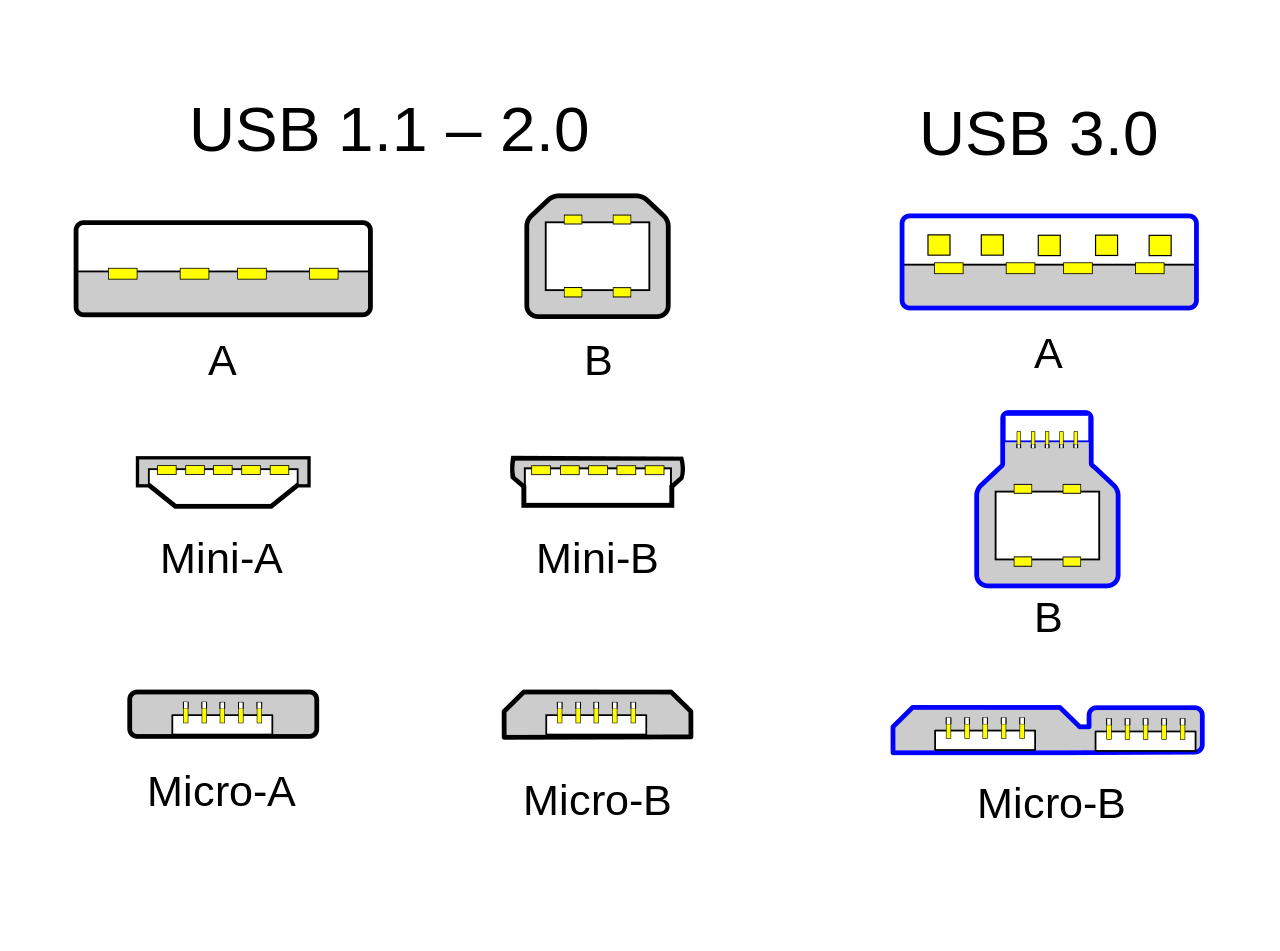
\includegraphics[width=0.6\textwidth]{images/usb_connectors.png}
    \caption{Connectors USB de tipus A i B. \cite{Contributors2024USB}}
    \label{fig:usb_connectors}
\end{figure}

\begin{itemize}
    \item Els connectors de tiups A son els que es connecten al dispositiu
    que actuarà com a mestre. Existeixen les variants \est{micro} i \est{mini},
    com es pot observar a la Figura \ref{fig:usb_connectors}, tot i que aquestes
    so son gaire populars. Amb l'aparició de l'estàndard \acro{usb3}, es van
    dissenyar nous connectors que fóssin compatibles amb els dels estàndards
    anteriors.
    \item Els connectors de tipus B son els que es connecten a l'esclau. Aquests
    també tenen les variants \est{micro} i \est{mini}, molt utilitzades
    en l'electrònica domèstica. També es va crear nous connectors de tipus B
    per a poder acollir l'estàndard \acro{usb3}.
    \item Finalment, els connectors de tipus C no tenen una jerarquia definida:
    serveixen per a dispositius que poden ser mestres o esclaus en diferents
    moments donats. La decisió de qui actua de mestre es pacta just a l'inici
    de la connexió, mitjançant un protocol específic \cite{Axelson2015USB}.
    Aquest connector, a diferència de la reta, és reversible: es pot connectar
    en les dues orientacions possibles. Es pot veure l'aspecte del connector
    a la Figura \ref{fig:usb_connectors_c}.
\end{itemize}

\begin{figure}[ht]
    \centering
    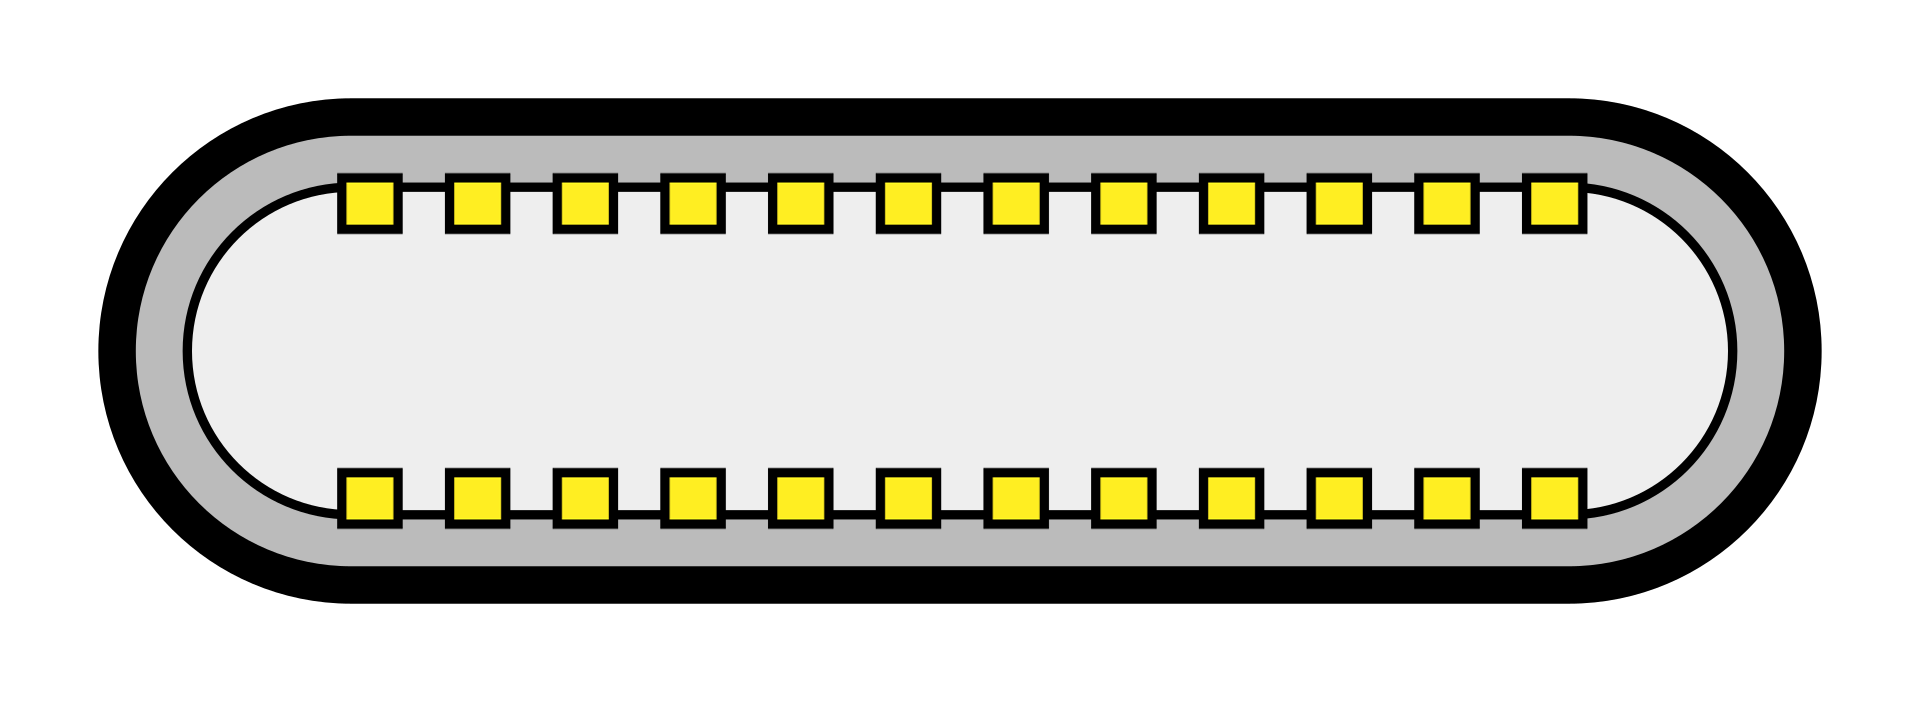
\includegraphics[width=0.3\textwidth]{images/usb_c.png}
    \caption{Connector USB de tipus C. \cite{Contributors2024USB}}
    \label{fig:usb_connectors_c}
\end{figure}

Així doncs, gairebé la totalitat de cables \acro{usb} seran de tipus A a tipus
B, utilitzant qualsevol format de mida. El tipus C, al ser bidireccional, pot
substituir el tipus A o el tipus B en els cables mencionats anteriorment.
Quan un cable només té un connector de tipus C en un cantó, no s'ha de pactar
la jerarquia de mestre-esclau, ja que ve definida pel tipus de connector a
l'altra banda del cable. Evidentment, també hi pot haver cables de tipus C a
tipus C.

Tanmateix, a l'any 2022 el Consell de la Unió Europea va aprovar una llei
que obliga un seguit de dispositius electrònics a utilitzar el connector
\acro{usb-c} enlloc d'altres estàndards \cite{Council2022Common}. Segons la
nota de premsa, el motiu d'aquesta llei és per a evitar més deixalla electrònica
per culpa de tenir diferents dispositius amb diferents connectors, així com
facilitar l'ús de les tecnologies als consumidors. Aquesta llei
es començarà a aplicar a finals de l'any 2024, i afectarà dispositius mòbils, 
alguns portàtils, tauletes, teclats i ratolins ina\l.làmbrics, entre
d'altres.

Sent el dispositu que es vol crear en aquest projecte un perifèric de
l'ordinador, la llei citada no l'afectaria. Tanmateix, la mateixa nota de premsa
informa sobre la intenció d'extendre aquest connector a altres dispositius.
Tenint present que el dispositiu que es vol crear podria entrar fàcilment en
aquest grup de perifèrics d'ordinador, s'ha decidit utilitzar un connector de
tipus \acro{usb-c} per a assegurar-nos la seva possible comercialització dintre
de la UE.

\chapter{Hardware}

En aquest capítol es detallarà tot el procés de realització del maquinari per
al projecte. La base teòrica del capítol anterior pot resultar de gran utilitat
per a entendre certes decisions preses durant algunes de les tasques d'aquest
capítol.

En aquest projecte es vol obtenir una placa de circuit imprès que permeti
transferir dades d'un sensor d'acceleració a l'ordinador, mitjançant la connexió
\acro{usb}. S'enviarà a producció la placa i es crearà un encapsulat senzill per
a evitar que aquesta es pugui omplir de pols o d'altres elements de l'entorn.
Finalment, es llicenciarà el disseny davant d'una entitat certificadora.

\section{Selecció del sensor}
\label{sec:sensor_selection}

El primer pas per a crear la placa és escollir quin sensor utilitzar. Per a
mesurar la inclinació d'un dispositiu es sol utilitzar un acceleròmetre.
Mitjançant un càlcul que es veurà més endavant i donades unes condicions es pot
determinar l'angle en relació a la direcció de la gravetat de la Terra \cite{PedleyTilt}.
Aquestes mesures es poden complementar amb un giroscopi, que ofereix més
precisió al sistema \cite{6702711}.

Després de fer una mica de recerca sobre els productes disponibles del mercat,
i tenint present la precisió que es necessita i el pressupost que es disposa,
s'ha trobat dues alternatives viables.

\begin{itemize}
    \item El sensors \est{ADXL3xx} es poden trobar a preus molt llaminers i
    comuniquen la lectura de l'acceleració en 3 dimensions mitjançant 3 línies
    analògiques. Per tant, la comunicació amb el microcontrolador serà el més
    senzilla possible \cite{adxl335}.
    \item El sensor \est{MPU6050}, en canvi, es comunica amb el microcontrolador
    mitjançant el protocol \acro{i2c}. Aquest protocol només necessita dues
    línies de comunicació, però implica implemenar una mica de lògica per a
    recuperar les dades. Tanmateix, aquest sensor també ofereix lectures de
    velocitat angular i temperatura, que podrien ser útils per a futures
    millores del projecte \cite{mpu6050specs}.
\end{itemize}

Així doncs, degut que el segon sensor és només pocs cèntims més car i ofereix
la possiblitat d'ampliar el projecte en un futur, s'utilitzarà el sensor
\est{MPU6050} per al sistema.

Aquest sensor es sol vendre amb una placa que estalvia connectar
certa electrònica i permet provar el sensor sense fer cap soldadura.
Aquest mòdul, anomenat \est{GY521}, es troba disponible a moltes botigues
d'electrònica, i s'ha decidit adquirir-ne un parell per al desenvolupament del
projecte. A la figura \ref{fig:gy521img} es pot veure l'aspecte d'aquest mòdul.

\begin{figure}[ht]
    \centering
    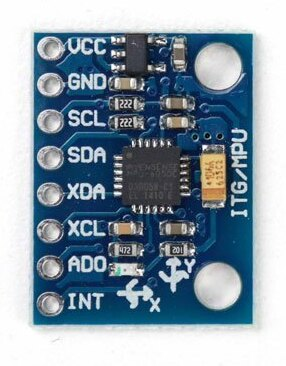
\includegraphics[width=0.3\textwidth]{images/modules/gy521img.jpg}
    \caption{Mòdul \est{GY521} \cite{gy521}.}
    \label{fig:gy521img}
\end{figure}

El circuit del mòdul \est{GY521} és lliure i es pot consultar a la figura
\ref{fig:gy521sch}. És prou senzill diferenciar la part utilitzada per a
convertir els 5V d'entrada en 3.3V per a alimentar a l'integrat de la resta
del circuit. Aquest mòdul també inclou un \acro{led} per a indicar que s'està
alimentant correctament.

Les connexions del lateral del mòdul fan molt còmode utilitzar-lo en entorns de
desenvolupament, on es connecten i desconnecten cables constantment. El fet
de disposar també d'un sistema funcional des d'un primer moment ajuda a
només centrar-se en la part de més alt nivell: l'aplicació del projecte.

\begin{figure}[ht]
    \centering
    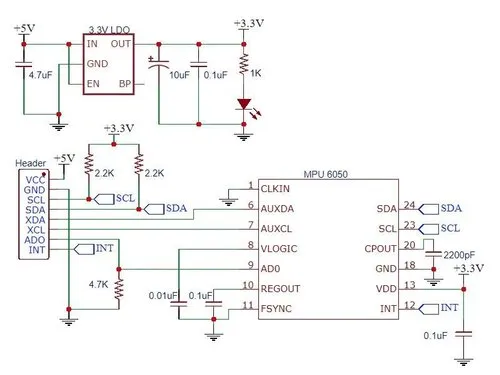
\includegraphics[width=0.6\textwidth]{images/modules/gy521sch.png}
    \caption{Esquema elèctric del mòdul \est{GY521} \cite{gy521}.}
    \label{fig:gy521sch}
\end{figure}

\section{Primer disseny}

En un primer moment es va decidir per utilitzar un microcontrolador que disposés
del perifèric \acro{usb} directament al maquinari, per a evitar programar-lo tot.
Tanmateix, es veurà que no s'acabarà utilitzant aquesta versió degut a motius
que s'explicaran més endavant. Dit això, s'ha decidit conservar aquest apartat
per a comprendre millor el procés de desenvolupament del projecte.

El microcontrolador que s'utilitzarà en aquesta versió és l'\acro{AtMega32u4}.
Aquest proporciona una interfície \acro{usb} integrada, i permet utilitzar la
interfície \acro{i2c} amb suficient facilitat. S'ha decidit utilitzar un
osci\l.lador extern per a generar un rellotge de freqüència $16MHz$
al microcontrolador \cite{AtMega32u4}.

\subsection{Esquemàtic}

El disseny de l'esquemàtic es basa en el disseny del mòdul \est{GY521} i es pot
consultar a la figura \ref{fig:sch_v1}. Tret del que s'ha comentat en els paràgrafs
anteriors, la resta de components i connexions no deixen de ser les evidents per
a un circuit amb aquestes característiques. Tot i això, s'ha decidit posar
èmfasi en alguns detalls on s'hi ha parat més atenció:

\begin{figure}[ht]
    \centering
    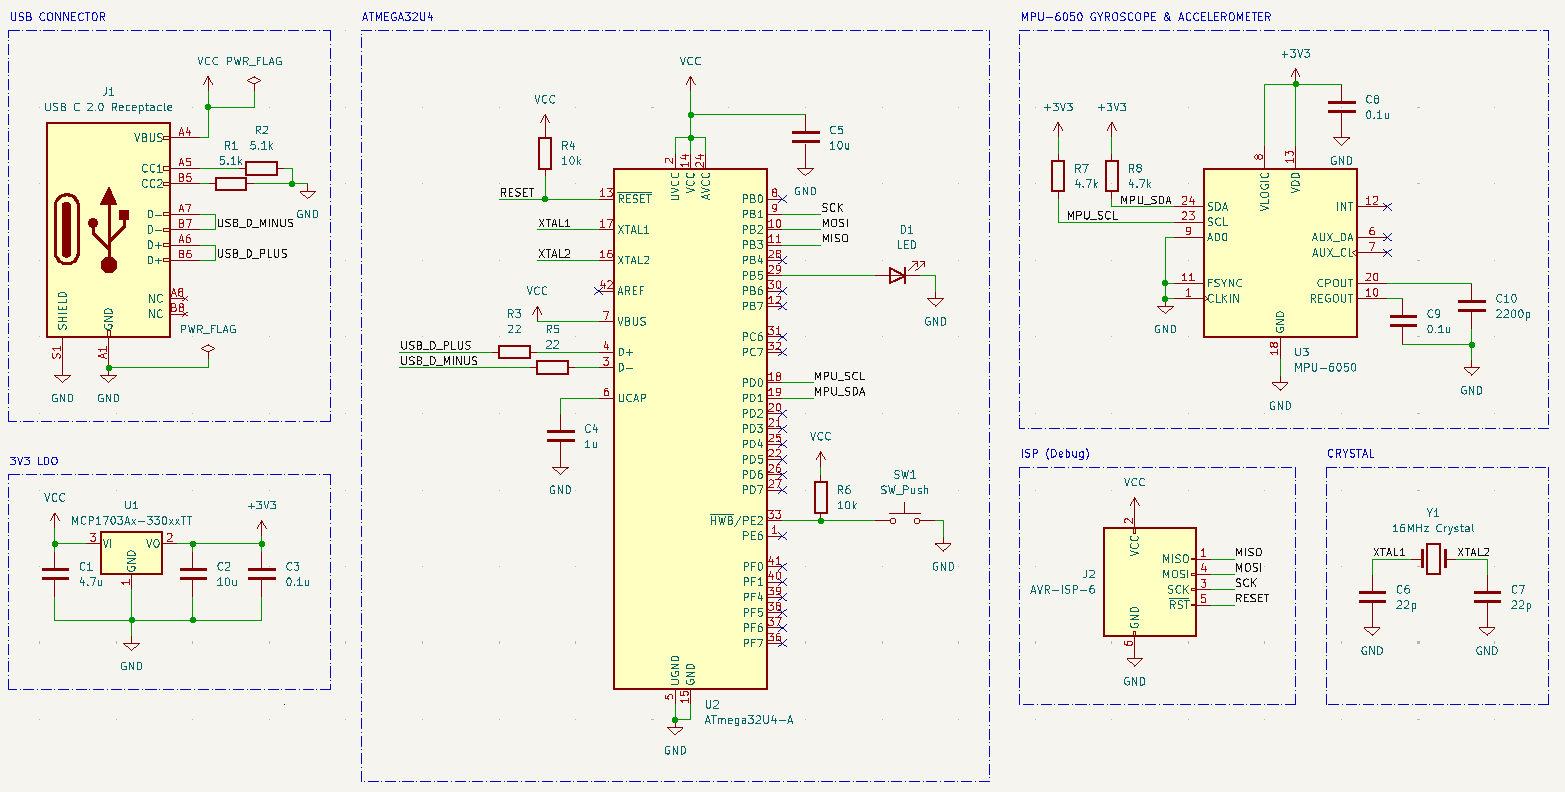
\includegraphics[width=0.9\textwidth]{images/kicad/gyro1_sch.png}
    \caption{Esquema elèctric de la primera versió.}
    \label{fig:sch_v1}
\end{figure}

\begin{itemize}
    \item Al costat de l'alimentació de cada integrat s'hi ha posat un
    condensador ceràmic de $10uF$ o $0.1uF$ (en funció del que recomanava
    cada fabricant al seu \est{datasheet}), per a assegurar-se que la tensió
    d'entrada és prou estable.
    \item S'ha hagut de posar un regulador lineal en el ciruit, ja que el
    sensor necessita estar alimentat a $3.3V$, però l'alimentació que proporciona
    el connector \acro{usb} és de $5V$.
    \item Al utilitzar un connector de tipus C, tot i communicar-se amb
    \acro{usb2}, hi ha un parell de cables extres que determinen a quina tensió
    s'ha d'alimentar el dispositiu. Tal i com es comenta en \cite{Axelson2015USB},
    si es desitja utilitzar una alimentació tradicional de $5V$ és suficient
    utilitzar dos \est{pull-downs} de 5.1kohms.
    \item El protocol \acro{i2c} necessita que les dues línies de comunicació
    estiguin amb \est{pull-ups}. Es veurà més endavant en el document el
    funcionament d'aquest protocol.
    \item L'esquema referent al cristall extern per al rellotge del microcontrolador
    és el recomanat pel fabricant en el mateix \est{datasheet} \cite{AtMega32u4}.
\end{itemize}

Cal destacar que, a diferència de la propera versió, aquest esquema sí que preveu
una connexió \acro{isp} per a programar la placa i un \acro{led} i polsador per
a interactuar d'una forma senzilla.

\subsection{Placa de circuit imprès}

Un cop acabat el disseny, utilitzant també el programa KiCad, es va començar a
crear la placa de circuit imprès. El procediment és prou senzill i es sol fer
de forma iterativa: crear un disseny molt dolent i anar-hi fent millores, fins
al punt on es considera que ja està prou bé (un disseny mai estarà perfecte).

A la figura \ref{fig:pcb_v1} es pot consultar la placa resultant. Com es pot veure,
no està del tot ben distribuida: això és perquè es va decidir canviar completament
de disseny abans d'haver-la acabat, i es va pensar que no valia la pena seguir
invertint temps amb un disseny que no veuria mai la llum.

\begin{figure}[ht]
    \centering
    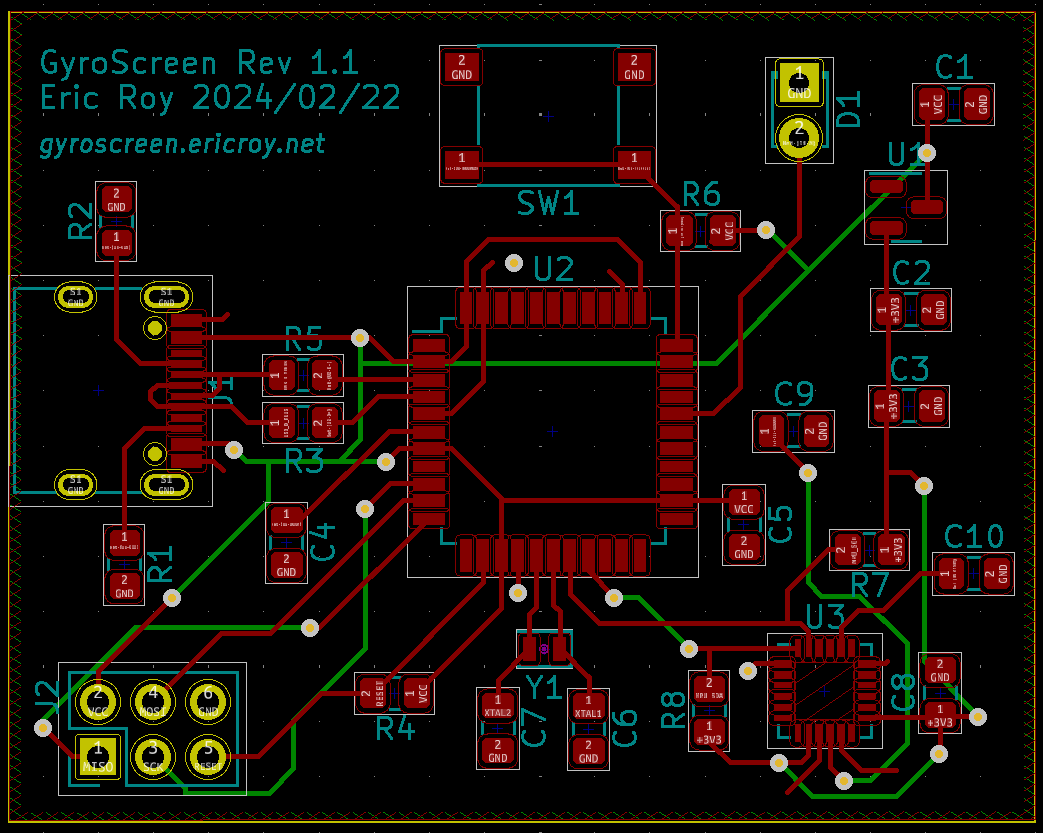
\includegraphics[width=0.8\textwidth]{images/kicad/gyro1_pcb.png}
    \caption{Placa de circuit imprès de la primera versió.}
    \label{fig:pcb_v1}
\end{figure}

\subsection{Problema del primer disseny}

Tal i com s'ha dit a l'apartat anterior, no es va acabar de dissenyar la placa
de circuit imprès degut al redisseny del \est{hardware}. El motiu es ben senzill,
no s'està utilitzant el microcontrolador adequat per al projecte.

Tal i com s'ha vist a l'esquemàtic, el microcontrolador només necessita 4 potes
per a informació (2 per \acro{usb} i 2 per \acro{i2c}). Això significa que es
deixaran al voltant de 20 entrades sense utilitzar. I no només això: aquest
microcontrolador disposa de molta més memòria de la que mai es necessitarà
\cite{AtMega32u4}.

El principal motiu per a fer el canvi és doncs el preu. Un \acro{AtMega32u4}
no és molt car \cite{AvrComparison}, però és més barat un dispotitiu \acro{avr} de la sèrie
\acro{AtTinyXX}, com es veurà en el segïuent apartat.

\section{Segona versió de la placa}

Tal i com s'ha comentat al final de l'apartat anterior, s'ha decidit apostar
per un microcontrolador més econòmic i senzill degut als pocs requisits que
demana el sistema. Després de fer una mica de recerca s'ha descobert la
família de microcontroladors \acro{AtTinyX5}, on la X pot variar en funció de
la memòria \est{flash} disponible \ref{AtTiny85}.

Aquests microcontroladors disposen de 8 potes, de les quals 2 són per
l'alimentació. Així doncs, de les 6 potes disponibles encara en sobraran dues
per si es vol afegir algun perifèric extra. Per a aquesta versió del projecte,
però, s'ha decidit no donar-hi cap ús.

Tanmateix, abans de produir una placa de circuit imprès, hi havia interès en
poder provar el microcontrolador per a assegurar-se que seria possible
realitzar el sistema amb aquest darrer. A través de recerca i recomanacions del
personal del laboratori de l'escola es va prendre coneixement de l'existència de
la placa \est{Digispark}.

\subsection{Proves amb \est{Digispark}}
\label{subsec:hw_digispark}

La placa \est{Digispark} es pot comprar a preus molt reduïts i a molts llocs.
És una placa de circuit imprès equipada d'un \acro{AtTiny85}, un connector
\acro{usb}, algun component per a regular les tensions, i tot de pins per a
poder connetar fàcilment qualsevol cable i component al microcontrolador
\cite{Digispark}. A la figura \ref{fig:digispark} es pot veure l'aspecte físic
de la placa.

\begin{figure}[ht]
    \centering
    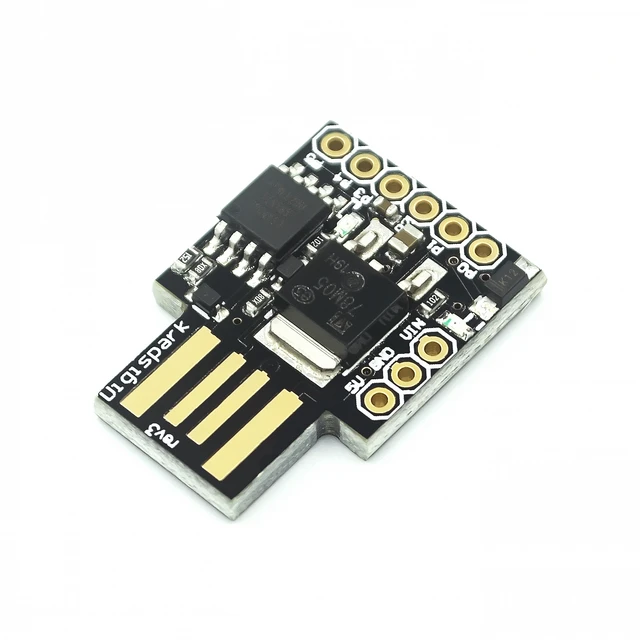
\includegraphics[width=0.3\textwidth]{images/modules/digisparkimg.png}
    \caption{Placa \est{Digispark} \cite{Digispark}.}
    \label{fig:digispark}
\end{figure}

Aquesta placa és de maquinari obert, i per tant, també es pot trobar fàcilment
el seu esquema elèctric. Es pot consultar a la Figura \ref{fig:digisparksch}
com el circuit és prou senzill, i només hi ha un parell de detalls que mereixen
la seva explicació, com podria ser l'ús de Díodes Zener. Es comentará en el
moment del disseny del propi circuit.

\begin{figure}[ht]
    \centering
    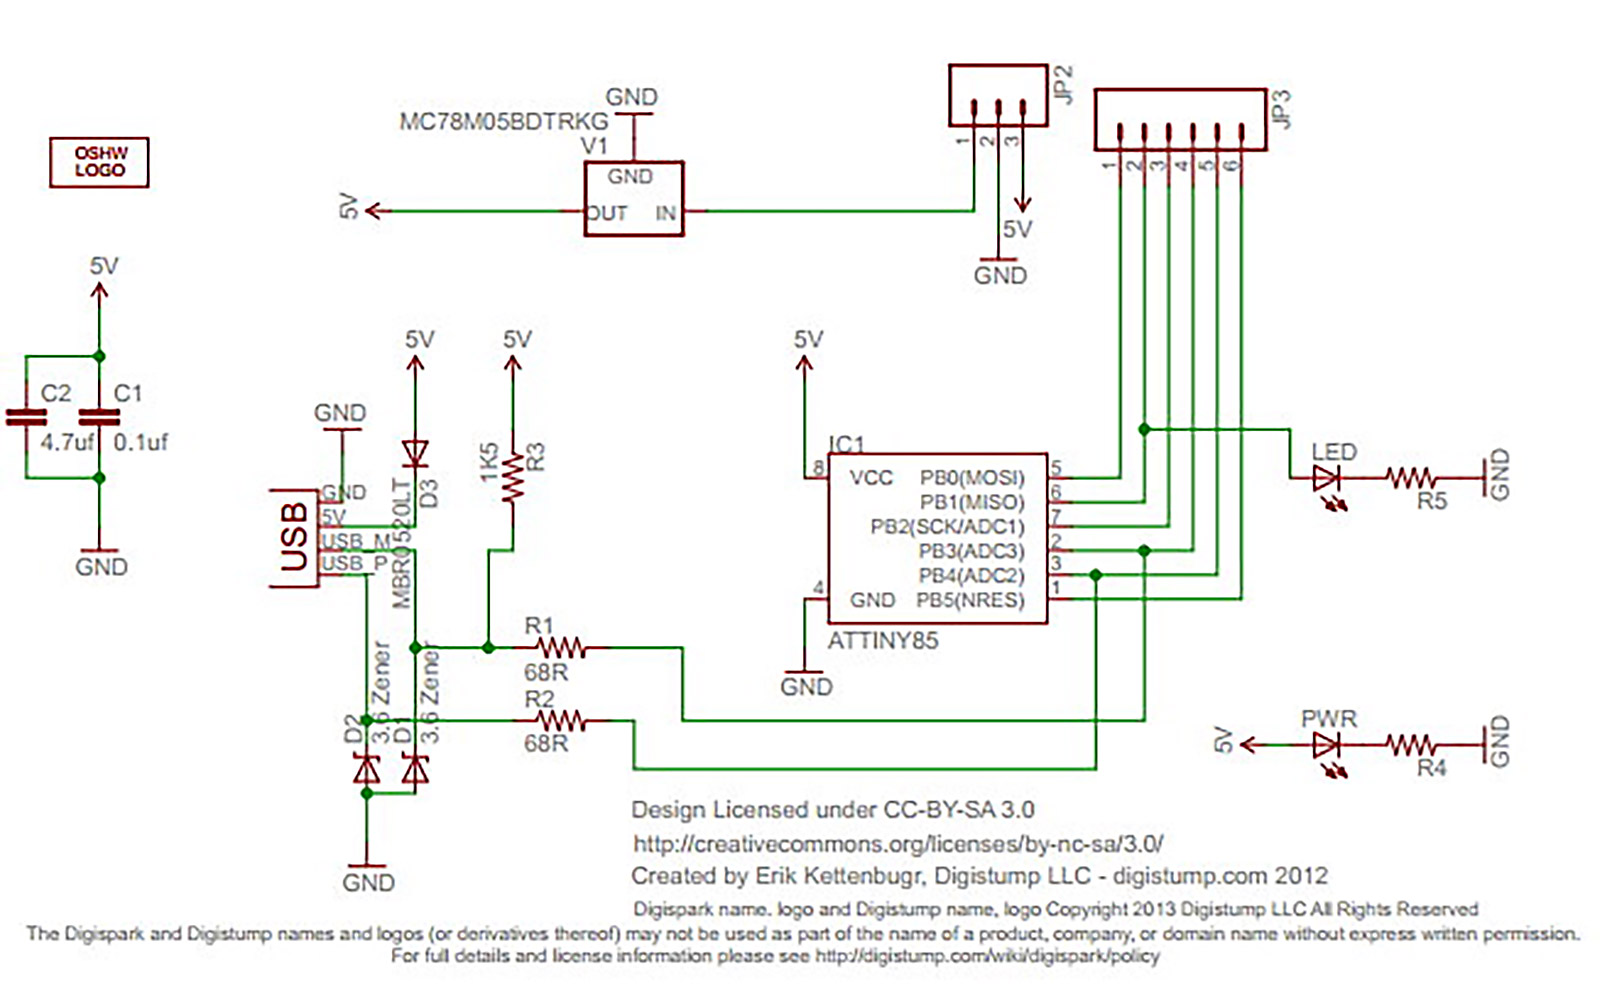
\includegraphics[width=0.8\textwidth]{images/modules/digisparksch.jpg}
    \caption{Diagrama de la placa \est{Digispark} \cite{Digispark}.}
    \label{fig:digisparksch}
\end{figure}

El microcontrolador ve programat amb un \est{bootloader} que utilitza la
llibreria \acro{v-usb} per a identificar-se com un port sèrie a l'ordinador
(és una de les sub-classes \est{hid}) i així poder programar-lo fàcilment.
És una placa bastant popular, de maquinari obert, i amb molta documentació i
tutorials disponibles per internet \cite{DigisparkBootloader}.

Es va adquirir un parell d'unitats d'aquesta placa, i es va connectar amb el
mòdul del sensor giroscopi. Mitjançant tutorials era senzill utilitzar la
placa \est{Digispark} com si d'un Arduino es tractés. Es podia, per exemple,
utilitzar la llibreria \est{LittleWire} per a comunicar-se amb el sensor amb el
protocol \acro{i2c} i llegir les dades necessaries.

Durant el transcurs d'aquestes proves també es va descobrir el projecte
\est{i2c\_tiny\_usb} \cite{I2cTinyUsb}. Aquest projecte ha aconseguit dissenyar una placa
molt semblant a la de \est{Digispark}, i mitjançant programari (tant del cantó
del microcontrolador com afegint contro\l.ladors al \est{kernel} de Linux),
el dispositiu s'identifica com un mestre \acro{i2c} de cara a l'ordinador, i
apareix a \verb|/dev/i2c-X| on X és el nombre de dispositiu.

Aquest projecte ha anat molt bé per a fer proves de precisió del sensor a més
alt nivell (per exemple, utilitzant la lliberria \acro{i2c} de Python). Tanmateix,
es va descartar utilitzar-lo per a aquest treball per a dos motius:

\begin{itemize}
    \item Aquest projecte pretén ser el màxim de versàtil possible i utilitzar
    els estàndards de més alt nivell. En el capítol anterior s'ha comentat que
    es volia utilitzar les classes \acro{hid} i el mòdul \acro{iio}. El projecte
    \est{i2c\_tiny\_usb} utilitza programari propi, i tot i que estigui inclòs
    en el \est{kernel} de Linux \cite{I2cTinyKernel}, s'hauria de fer de zero per altres sistemes
    operatius.
    \item L'objectiu del projecte és aprendre durant el procés de desenvolupament.
    Si s'agafa un projecte que ja ho té tot fet no s'adquirirà experiència en
    aquests camps.
\end{itemize}

Així doncs, s'ha acabat utilitzant la placa \est{Digispark} per a validar
que el projecte es podria desenvolupar en aquest maquinari, i un cop es va
conéixer la bona notícia es va començar a desenvolupar la pròpia placa de circuit
imprès.

\subsection{Esquemàtic}

L'esquemàtic d'aquesta segona versió no té molts secrets. Consisteix en agafar
el circuit de la versió anterior i canviar tot el que té a veure amb l'antic
microcontrolador per al nou. S'ha utilitzat com a referència el circuit de la
placa \est{Digispark}, tenint en compte que algunes coses, com el regulador de
tensió extern, no son necessaries per a aquest projecte \cite{Digispark}.

En aquest nou circuit s'utilitza el rellogte intern del microcontrolador, que
ja s'ha vist que és suficient per a comunicar-se per \acro{usb}. Només hi ha
una novetat a comentar en aquesta segona versió, i és la presència de dos
díodes Zener en les línies d'\acro{usb}. El motiu rau en el protocol \acro{usb}:
tot i estar alimentat a $5V$, les línies de dades funcionen a $3V3$. Tal i com
s'ha comentat a l'apartat \ref{subsub:usb_physic}, els dos díodes asseguren
que la tensió mai supera aquest llindar.

\begin{figure}[ht]
    \centering
    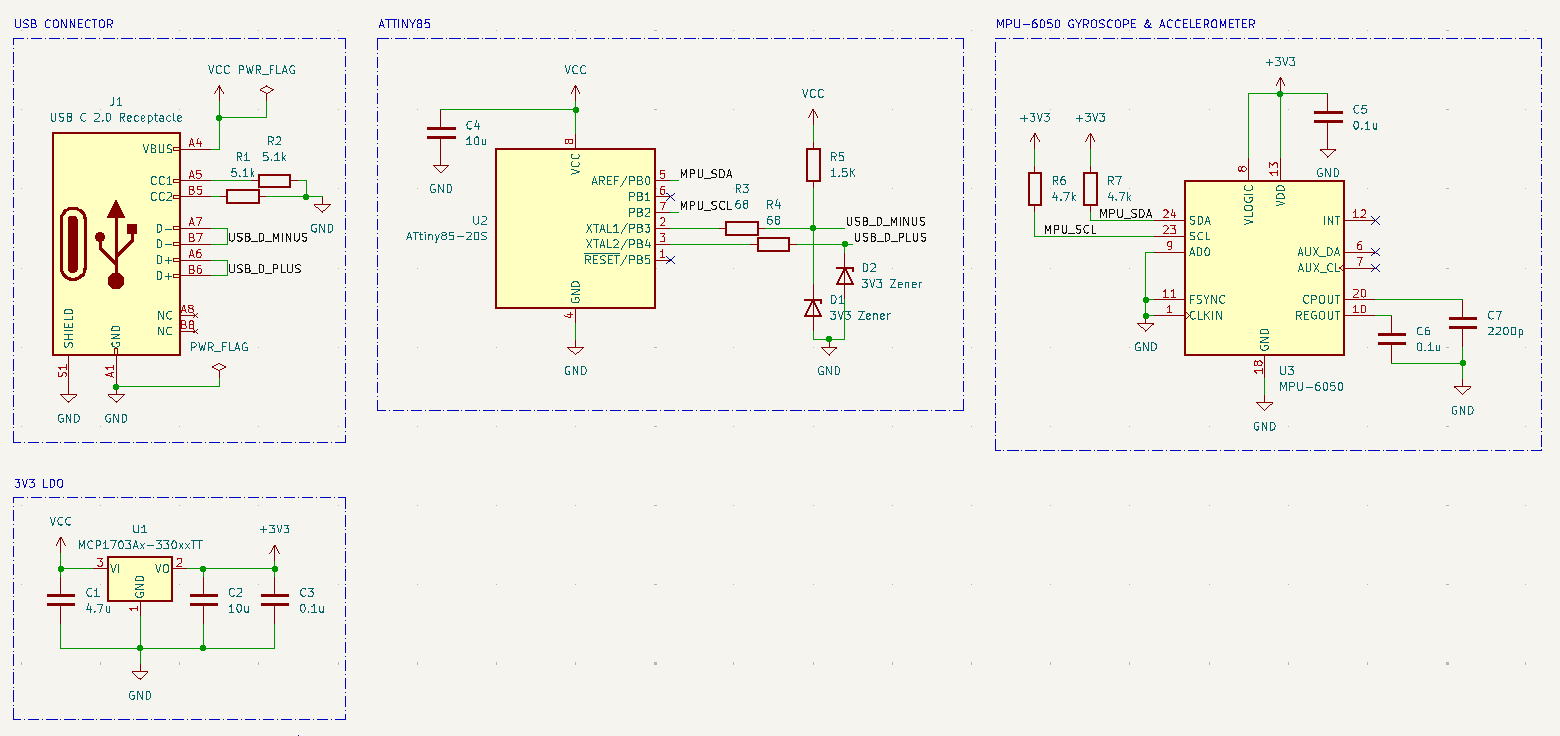
\includegraphics[width=1\textwidth]{images/kicad/gyro2_sch.png}
    \caption{Esquema elèctric de la segona versió.}
    \label{fig:sch_v2}
\end{figure}

Finalment, s'observa que en el diagrama de la figura \ref{fig:sch_v2}
no hi ha cap element amb el que una
persona pugui interactuar directament amb el dispositiu (polsador, llum, ...).
Això és a propòsit, ja que es pretén que el dispositiu acabi tancat en una capsa
i que l'usuari no hagi de tocar-lo mai.

\subsection{Placa de circuit imprès}

Un cop creat l'esquema elèctric, s'ha pogut començar a dissenyar la placa de
circuit imprès, de la mateixa manera que amb la versió anterior. Una de les
tasques més difícils d'aquest procés és escollir \est{footprints} de components
que estiguin actualment en estoc, i assegurar-se que les línies de tensió
són una mica més groixudes que la resta. A la figura \ref{fig:pcb_v2}
es pot veure el resultat
final d'aquest segon disseny.

\begin{figure}[ht]
    \centering
    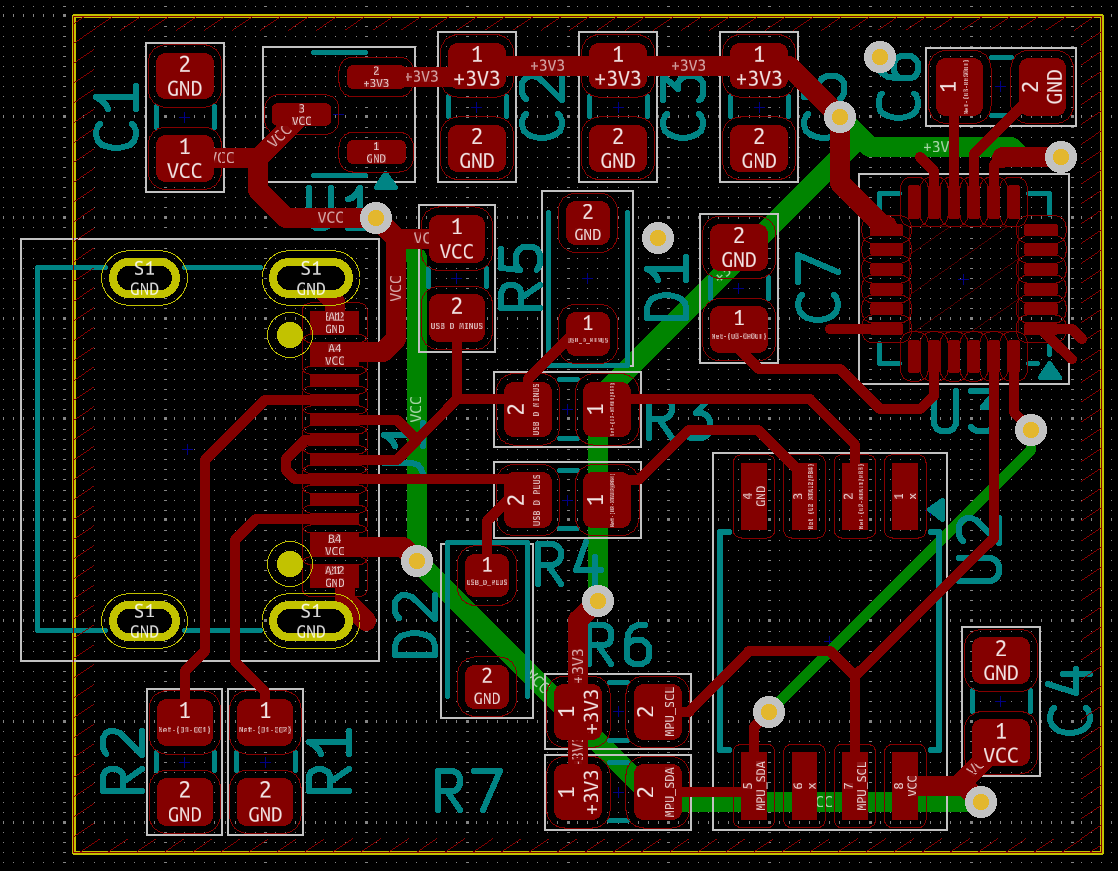
\includegraphics[width=0.75\textwidth]{images/kicad/gyro2_pcb.png}
    \caption{Placa de circuit imprès de la segona versió.}
    \label{fig:pcb_v2}
\end{figure}

S'ha utilitzat,
sempre que ha sigut possible, components amb \est{footprints} de dimensions 0805,
ja que amb aqeusta mida es poden soldar a mà. Tot i que no s'ha previst afegir
manualment els components, el fet d'escollir aquestes mides és una assegurança
que si s'espatlla o es crema algun component, aquest es podrà canviar.
Evidentment, en un disseny per a produir-se en massa es pot reduir la mida dels
components.

Com que a la part de darrere de la placa només hi ha d'anar un parell de vies,
però cap component, s'ha decidit afegir-hi els crèdits del projecte: autor,
titulació, logos de l'escola i de maquinari lliure, i enllaç a una possible
pàgina web.

Tot i haver parat atenció amb els components, es veurà en el següent apartat que
l'empresa amb qui s'ha encarregat la producció de la placa no tenia disponibles
alguns d'aquests. Així doncs, s'ha hagut de fer una nova revisió amb petites
modificacions d'alguns components.

\subsection{Producció de la \acro{pcb}}

Amb la placa de circuit imprès ja preparada, només faltava produir-ne algunes
unitats. Per recomanacions de la universitat s'ha optat per utilitzar el
proveïdor \acro{jlcpcb}. Aquest ofereix bons preus, plaços curts i també té el
servei de muntatge de la placa (és a dir, soldar-hi tots els components)
\cite{JlcPcb}.

Degut al poc talent i ganes que hi havia en soldar un per un els components, i
sabent que alguns són molt petits i seria senzill cometre errors, s'ha optat
per delegar aquesta tasca al proveïdor. Evidentment, el cost de muntatge ha
sigut el més elevat de tota la comanda, però imprimir i muntar 5 plaques
ha sortit per menys de 100€, enviament i \acro{iva} inclosos.

\begin{figure}[ht]
    \centering
    \begin{subfigure}{0.45\textwidth}
        \centering
        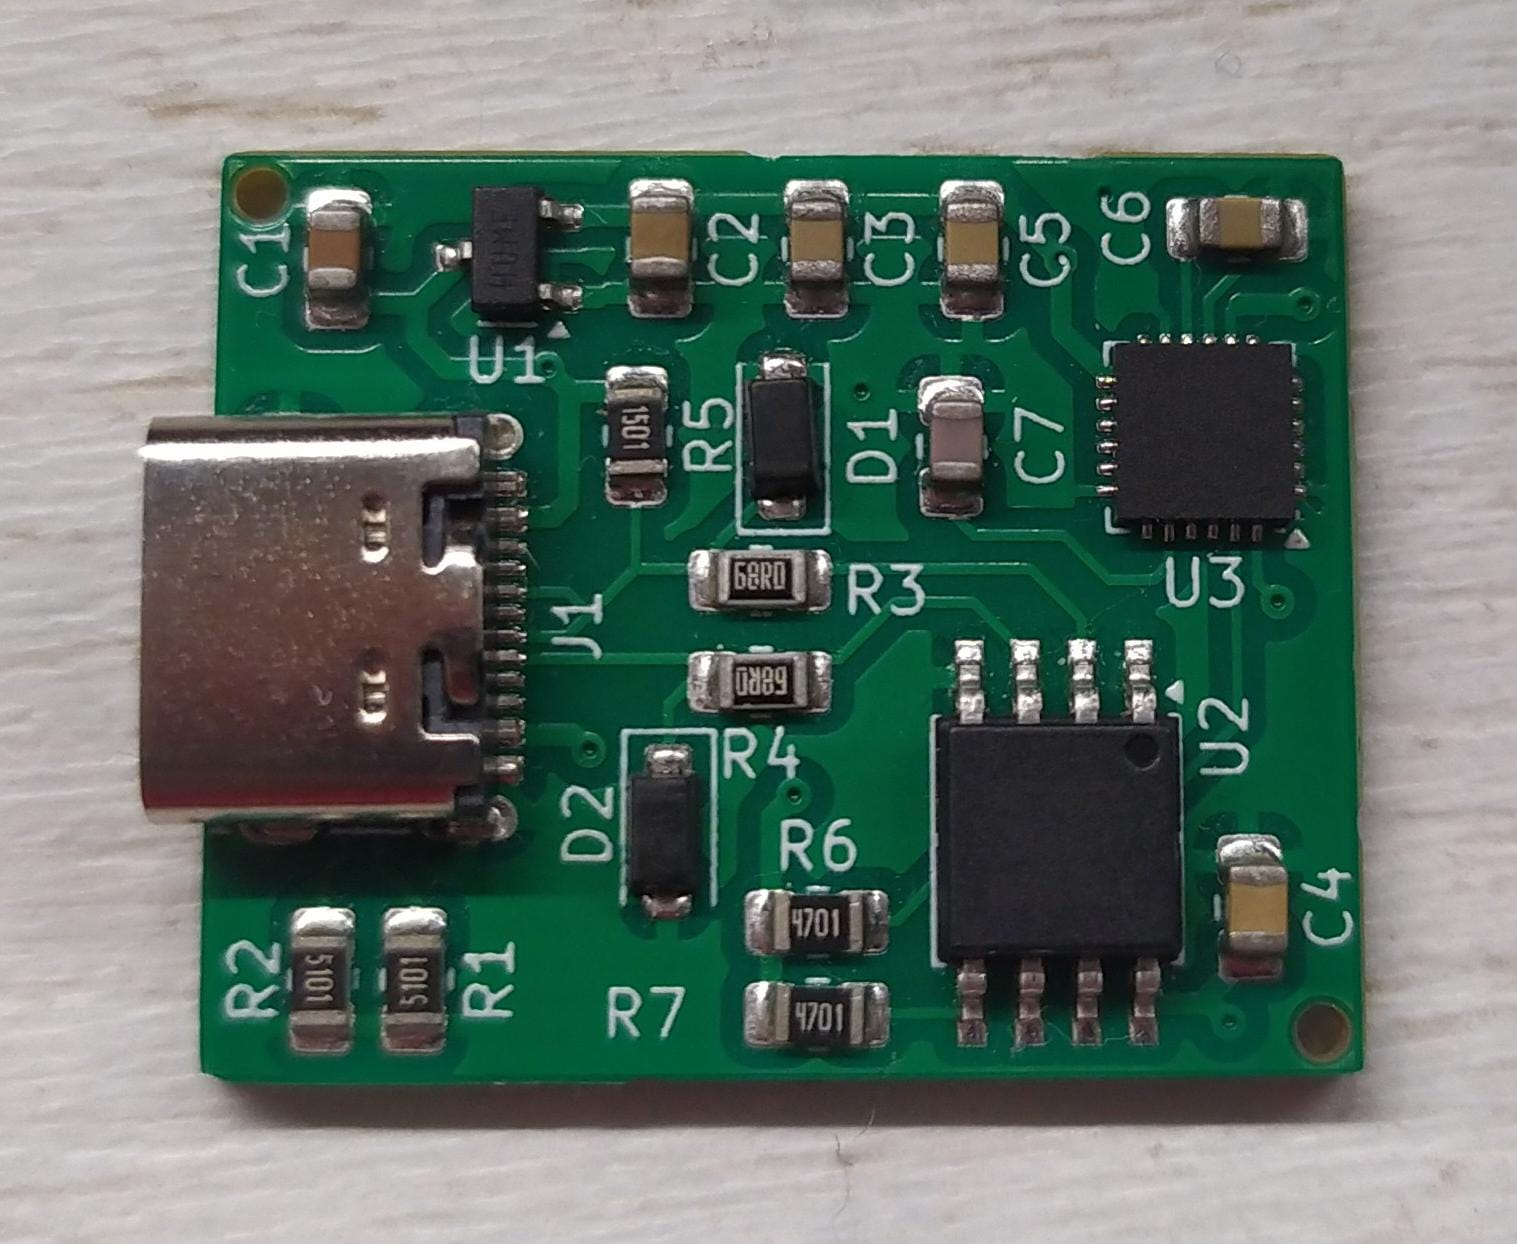
\includegraphics[width=0.9\textwidth]{images/device/top.jpeg}
        \caption{Cara superior.}
        \label{fig:printedpcb_top}
    \end{subfigure}
    \begin{subfigure}{0.45\textwidth}
        \centering
        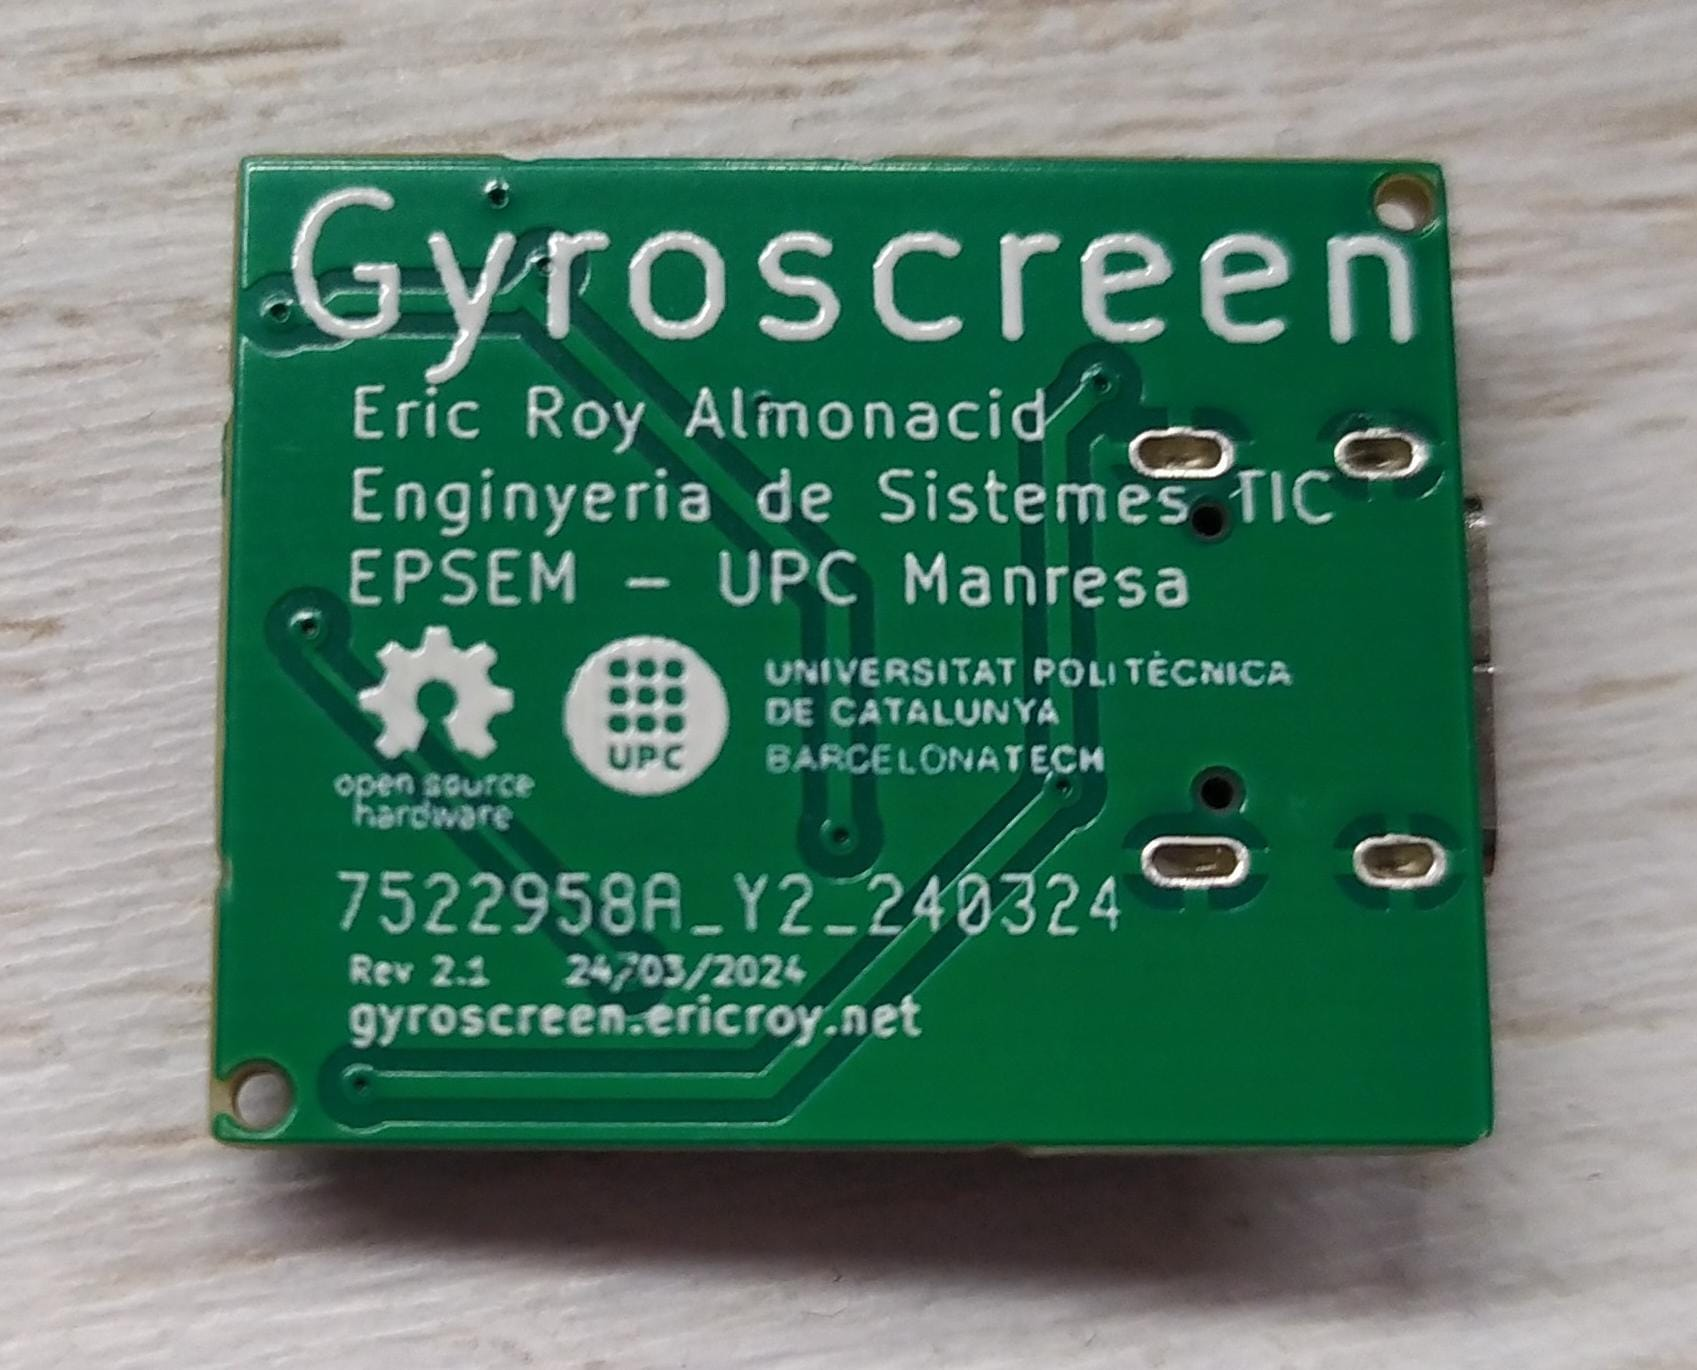
\includegraphics[width=0.9\textwidth]{images/device/bottom.jpeg}
        \caption{Cara inferior.}
        \label{fig:printedpcb_bottom}
    \end{subfigure}
    \caption{Placa de circuit imprès del projecte.}
    \label{fig:printedpcb}
\end{figure}

El resultat final ha quedat molt professional i es pot veure a la figura
\ref{fig:printedpcb}. Es pot veure també com s'ha aprofitat la cara inferior
per a afegir els crèdits del projecte.

\section{Encapsulat}

Quan es va saber que la placa impresa ja no rebria més modificacions físiques,
es va decidir crear una petita carcassa per a evitar que hi entri pols o les
ditades el puguin fer malbé. En un futur, aquesta carcassa també podrà protegir
al dispositiu d'altres agents externs, però en el moment del disseny l'objectiu
era tenir cura del dispositiu durant la fase de desenvolupament.

Així doncs, es va utilitzar el programa \est{FreeCAD} per a dissenyar una
carcassa amb dues peces: una superior i una inferior. Aquestes encaixarien entre
sí i, amb l'ajuda de cola quedarien subjectes. Les mesures s'han pres a partir
del model de \est{KiCad}, però també s'han corroborat amb la placa física i un
peu de rei.

A la figura \ref{fig:3d_freecad} es poden veure les dues parts dissenyades. Com es pot
apreciar, només s'hi ha deixat un forat per a permetre el pas del connector
\acro{usb}. S'ha utilitzat parets de 1.5 mm, i un marge entre les dues peces de
0.25 mm.

\begin{figure}[ht]
    \centering
    \begin{subfigure}{0.40\textwidth}
        \centering
        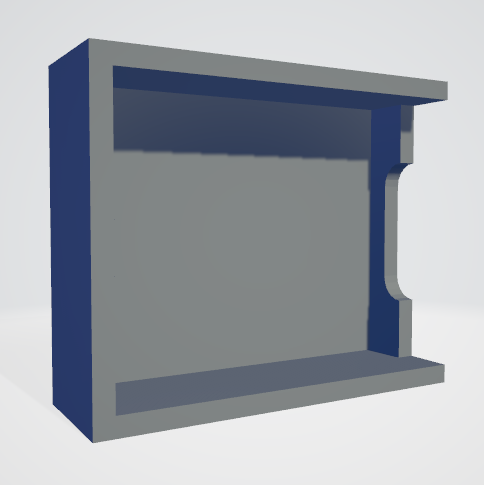
\includegraphics[width=0.9\textwidth]{images/freecad/3d_bottom.png}
        \caption{Part inferior.}
        \label{fig:3d_freecad_bottom}
    \end{subfigure}
    \begin{subfigure}{0.4\textwidth}
        \centering
        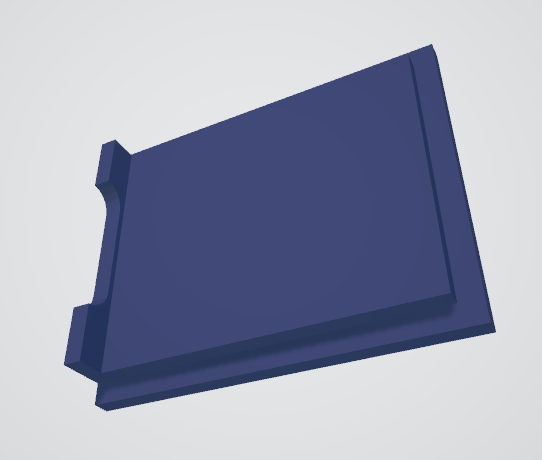
\includegraphics[width=0.9\textwidth]{images/freecad/3d_top.png}
        \caption{Part superior.}
        \label{fig:3d_freecad_top}
    \end{subfigure}
    \caption{Disseny 3D de l'encapsulat.}
    \label{fig:3d_freecad}
\end{figure}

Es va aconseguir imprimir les dues peces amb una de les impressores de
l'escola, i es va aconseguir el resultat que es pot apreciar a la figura
\ref{fig:3d_real}. Finalment, es va comprovar que totes les peces encaixaven a la
perfecció i la placa cabia a dintre de la carcassa.

\begin{figure}[ht]
    \centering
    \begin{subfigure}{0.50\textwidth}
        \centering
        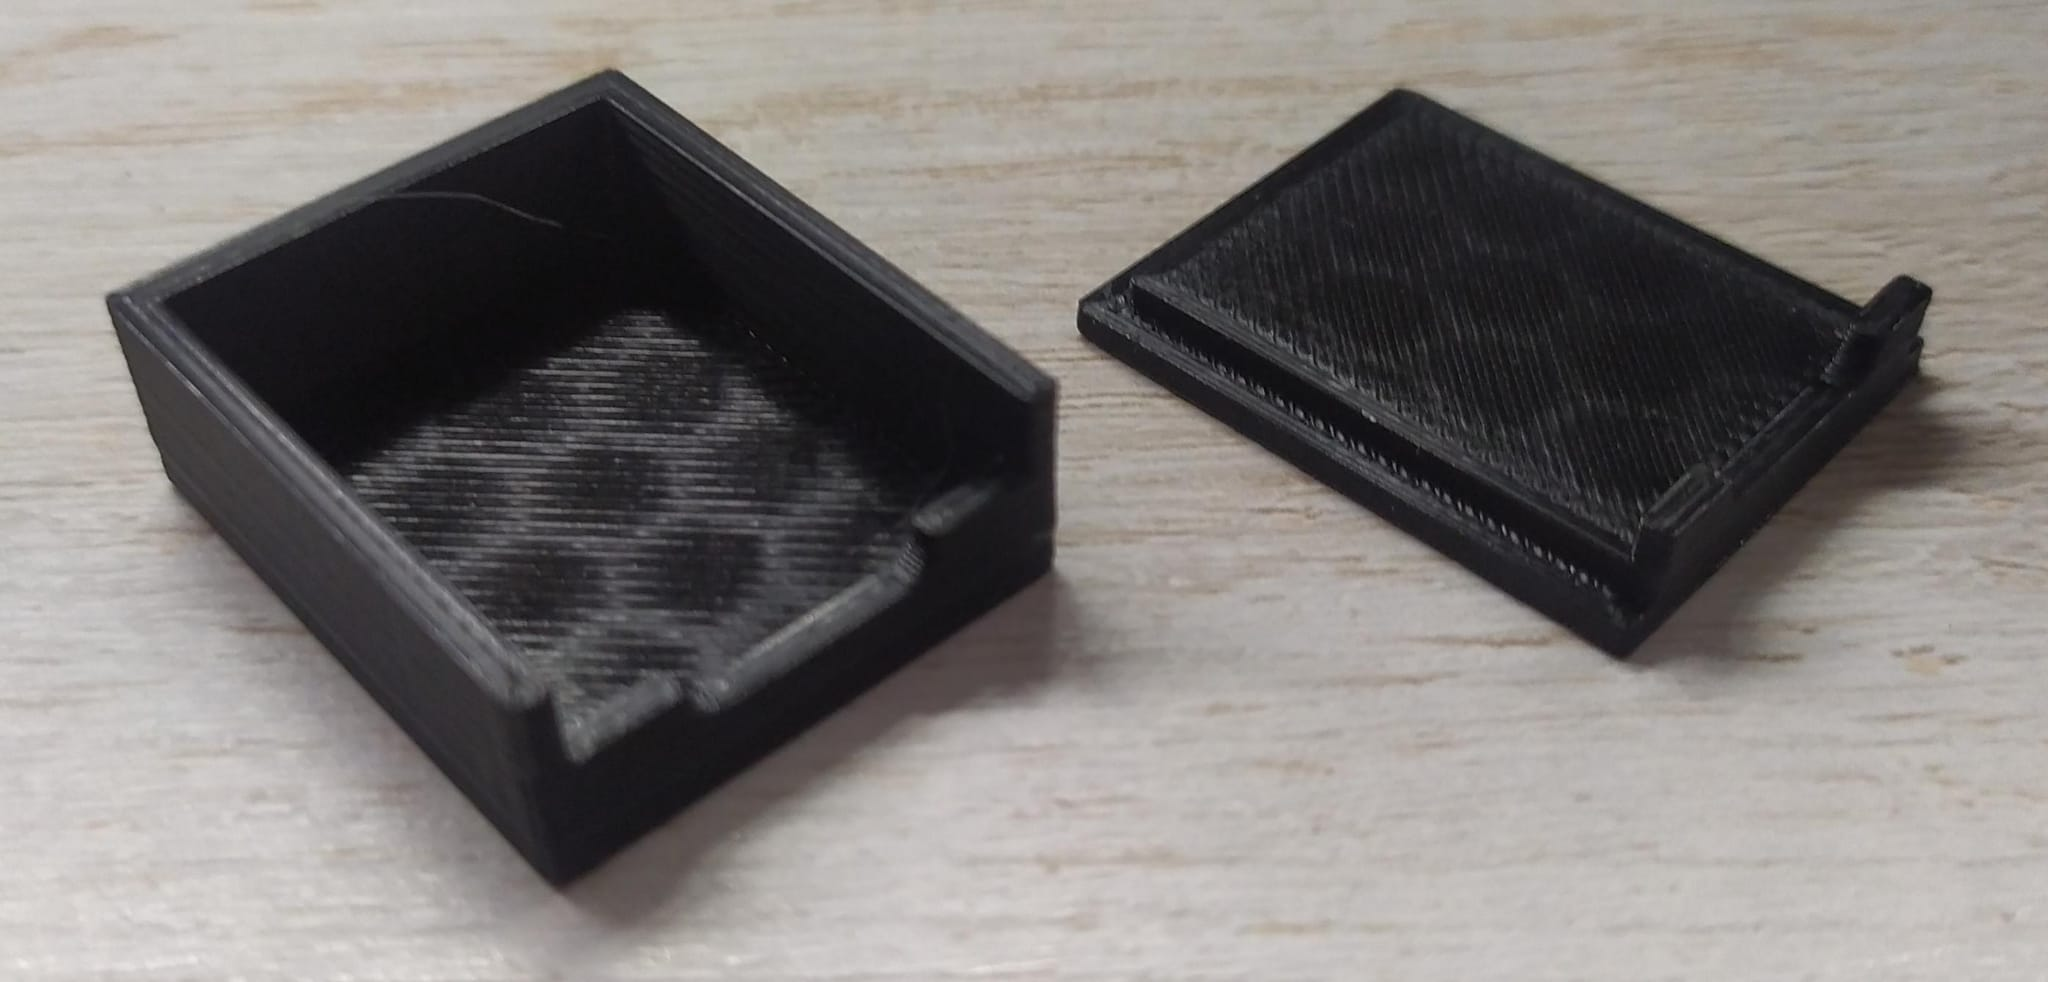
\includegraphics[width=0.9\textwidth]{images/device/3d_unmounted.jpeg}
        \caption{Sense muntar.}
        \label{fig:3d_real_unmounted}
    \end{subfigure}
    \begin{subfigure}{0.4\textwidth}
        \centering
        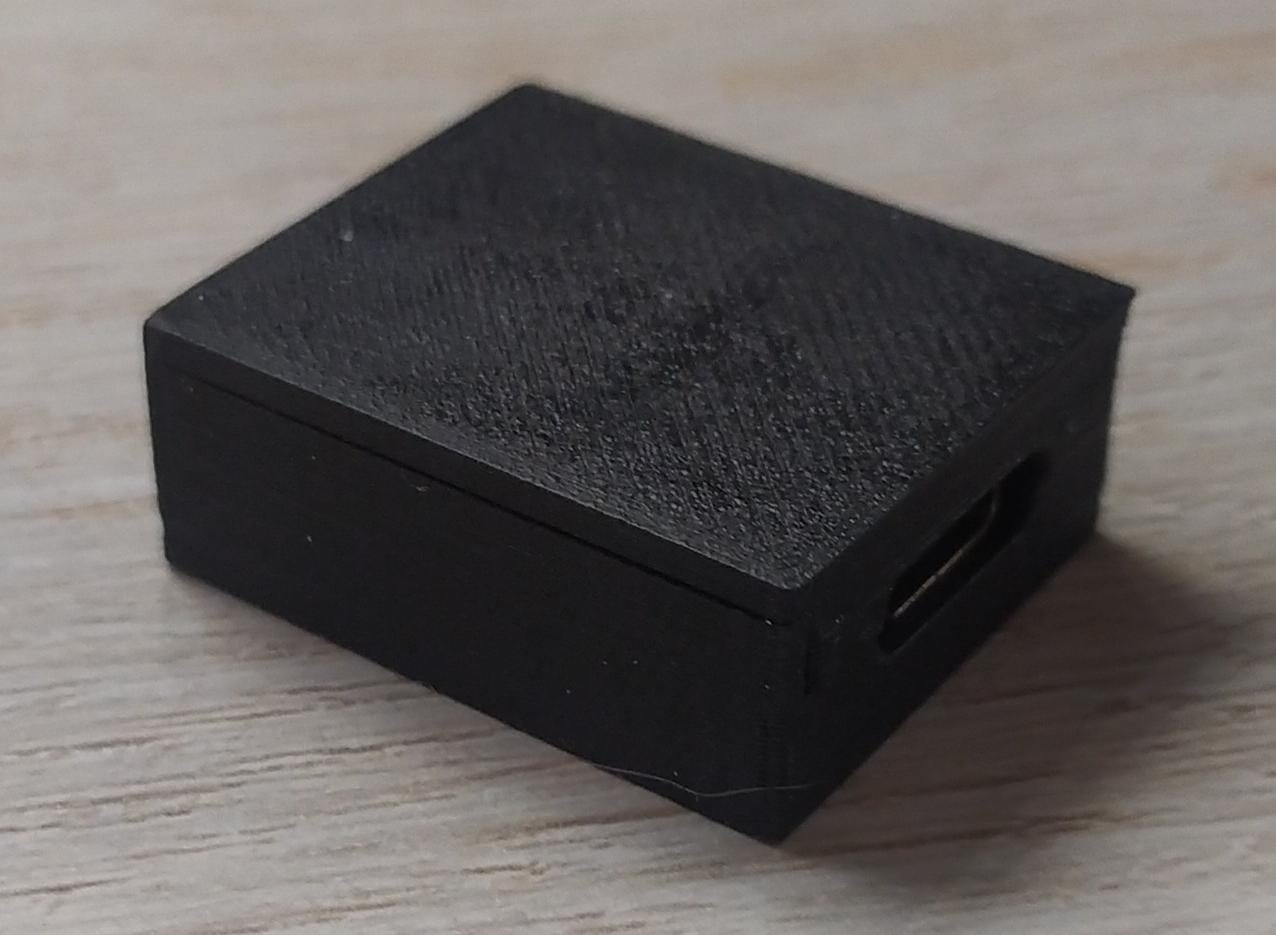
\includegraphics[width=0.9\textwidth]{images/device/3d_mounted.jpeg}
        \caption{Muntat.}
        \label{fig:3d_real_mounted}
    \end{subfigure}
    \caption{Disseny 3D de l'encapsulat.}
    \label{fig:3d_real}
\end{figure}

\section{OSHWA}

Un cop es va saber que el disseny físic del projecte era defintiu, es va decidir
publicar-lo a \acro{oshwa}. L'\est{Open-Source HardWare Association} és, com el
nom indica, una associació que vetlla pel maquinari de codi obert. Una de les
diverses tasques que fa és mantenir un registre de dissenys de maquinari obert,
sempre que els autors ho autoritzin \cite{Oshwa}.

Un dels beneficis de registrar el disseny en el seu sistema és que queda una
evidència (més) que el projecte s'ha fet, té la llicència que té, i protegeix
a l'autor contra possibles plagis. El més interessant de tot això és que aquest
servei s'ofereix gratuïtament: l'associació accepta donacions, però no son
necessàries per a poder registrar un disseny.

Així doncs, es va registrar el dispositiu a la seva base de dades i, després
de omplir el formulari i aquest ser revisat per l'associació, el dispositiu
va ser acceptat i es troba actualment sota la llicència \verb|ES000045|.
A la figura \ref{fig:oshwa} es troba el logo que es pot incloure al projecte,
com a resultat d'aquesta certificació.

\begin{figure}[ht]
    \centering
    
\includegraphics[width=0.5\textwidth]{images/oshwa.png}
    \caption{Certificació \acro{oshwa} obtinguta per al projecte.}
    \label{fig:oshwa}
\end{figure}


\chapter{Firmware}
\section{i2c on littlewire}
whatchdog
osccal
\section{canvi a accel3d}
\section{PID-VID}

\chapter{\est{Software} a Linux}

La darrera peça del puzzle per a que el sistema pugui funcionar és el
programari del cantó de l'ordinador. Tal i com s'ha comentat al capítol
\ref{cap:estat-de-l-art}, el fet d'utilitzar \acro{iio} implica que el
programari que es disseny per Linux no serà compatible amb la resta de
sistemes operatius. També s'ha vist que \est{Xlib} només existeix en sistemes
basats en Linux.

Així doncs, aquest capítol té per objectiu dissenyar un programari senzill però
robust per a poder utilitzar el sistema en dispositius basats en Linux. Es
centraran les proves en la distribució de Linux \est{Ubuntu}, concretament en
les versions 18.04 i 24.04 \acro{lts} (\est{Long-Term Support}), però tot hauria
de funcionar de la mateixa forma amb la resta de distribucions.

\section{Punt de partida}

Un bon inici per a aquesta part del projecte és identificar què és el que
s'espera del programa: com s'ha d'insta\l.lar, com ha de funcionar i com
s'ha de configurar. D'aquesta forma, es veu els requisits del programa des del
punt de vista d'un usuari, fent sovint més senzill l'ús de l'aplicació.

Després de donar-hi algunes voltes s'ha decidit utilitzar Python per a
desenvolupar l'aplicació, degut a la gran disponibilitat de llibreries, el fet
que ja es troba insta\l.lat per defecte en moltes distribucions de Linux, i
la simplicitat de programació (en comparació als llenguatges de baix nivell).
S'ha decidit també aque s'utilitzarà un servei de Linux per al programa principal.
Això implicarà alguna configuració addicional, però de ben segur que facilitarà
la vida als usuaris.

Un altre aspecte important del programa és la manera de configurar-lo. Tot i que,
idealment, el millor per als usuaris finals seria una interfície interactiva,
Linux sol funcionar amb fitxers per tot. Així doncs, s'ha decidit crear un fitxer
\verb|.conf| per a guardar les configuracions de l'aplicació. Aquest fitxer té
un format pactat i descrit a la documentació del programa, i es podrà guardar en
diferents llocs específics del sistema, on el progrma els buscarà. Crear una
interfície interactiva que modifiqui aquest fitxer no hauria de ser una tasca
gens complicada, i podria ser una perfecta ampliació al sistema.

Pel que fa a l'insta\l.lació, es dissenyarà un paquet de Debian (una de les
distribucions de Linux més populars) que insta\l.larà els requisits i configurarà
el que faci falta per al bon funcionament del programa, fent aquesta tasca
possible per a persones que no dominin tant la línia de comandes.

\section{Llibreries utilitzades}

Un cop es sap les tasques que s'haurà de fer és el moment de cercar si hi ha
alguna eina que pugui simplificar la tasca de desenvolupament. Tal i com s'ha dit
a l'apartat anterior, Python té moltes llibreries (o mòduls) creats per la
comunitat i disponibles per tothom. Coneixent les parts més difícils de
l'aplicació, es pot cercar si algú ja les ha implementat.

\subsection{\est{PyLibiio}}

El primer mòdul cercat és \est{PyLibiio}, que consisteix en la llibreria de
Linux \est{libiio} portada a Python. CITE REPO. La llibreria compilada acostuma
a estar insta\l.lada per defecte en la majoria de sistemes basats en Linux, però
la portabilitat a Python és un afegit que s'ha d'insta\l.lar.

Ja s'ha comentat en el capítol \ref{cap:estat-de-l-art} la importància
i beneficis d'utilitzar l'entorn de \acro{iio} per al programa d'aquest projecte,
així que si, a més a més, es pot fer des de l'alt nivell d'abstracció que ofereix
Python, encara millor.

Aquest mòdul no té molta complexitat, i menys si es segueix com a referència
algun dels exemples llistats. La majoria dels exemples consistien en replicar
amb Python les comandes d'exemple de la llibreria \est{libiio}.

Tanmateix, durant les proves de l'exemple de la comanda \verb|iio_info| s'ha
vist que aquesta no donava els mateixos resultats que el mateix programa implementat
en C. Quan no s'especifica cap argument en la línia de comandes, s'hauria 
d'utilitzar el primer grup de dispositius possible. En canvi, el programa d'exemple
s'aturava sense mostrar cap error.

Així doncs, amb la intenció de contribuir a millorar el projecte, es va
notificar de l'error i es va crear una \est{Pull Request}, és a dir, es va
proposar una solució. CITE Aquesta encara està pendent d'aprovació (ja que sembla que
les persones encarregades de mantenir la llibreria no tenen molt de temps
disponible).

\subsection{\est{PyLibudev}}

Durant el desenvolupament del programa es va veure la necessitat d'obtenir el
número de sèrie a partir de l'adreça d'un dispositiu \acro{iio}. Després de fer
recerca, es va veure que la forma més senzilla era utilitzant una comanda
de \acro{udev}. I, com no podia ser d'una altra manera, es va cercar si es podia
estalviar aquesta comanda i utilitzar una llibreria de Python en el seu lloc.

És important evitar utilitzar comandes ja que aquestes són més propenses a
variar i deixar de funcionar que la pròpia interfície de desenvolupament que
proporcionen les llibreries, com és el cas de \est{libudev}. Per aquest motiu,
quan es va conéixer l'existència de \est{PyLibudev} es va fer el canvi en la
implementació. CITE

Aquesta llibreria també disposava d'exemples, i no s'hi ha trobat cap
error aparent. Com també ha passat amb el mòdul anterior, la pròpia llibreria
ja ve insta\l.lada, però la portabilitat a Python s'ha de llistar com una
dependència del programa.

Quan encara no es sabia del tot segur si es faria servir \acro{iio} o, una capa
més per sota, el protocol \acro{hid}, també es va cercar si hi havia una
implementació per Python de la llibreria \est{libhid}. Es va trobar el mòdul
\est{PyLibhid}, un projecte molt complet amb, fins i tot, eines per a debugar
interactivament dispositius \acro{hid}. Finalment es va descartar utilitzar
aquest afegit, ja que es va passar a utilitzar \acro{iio}.

\subsection{\est{PyXrandr}}

Finalment, la tercera i última contribució externa de l'aplicació és el
mòdul \est{PyXrandr}. A diferència de la resta, aquest mòdul no es troba
disponible al repositori oficial de Python \est{PyPi} i, per tant, no es pot
insta\l.lar amb la comanda \est{pip3} o marcar com a dependència quan es crei
l'aplicació final.

Aquest projecte, disponible a \est{GitHub}, és una abstracció de la comanda
\est{xrandr} CITE. S'ha vist en l'apartat \ref{subsec:xrandr} que la llibreria
\est{Xlib} pot ser una mica complicada d'utilitzar, i aquesta comanda no ha
canviat gaire en bastant temps. Així doncs, es considera una bona alternativa
per a l'aplicació.

La persona que va desenvolupar \est{PyXrandr} en un primer moment ha deixat de
mantenir el projecte. A més a més, aquest no va tenir en compte tots els casos
d'ús, deixant en el codi alguns errors. Ja hi ha gent que ha creat \est{forks}
(còpies del projecte) i \est{pull reuquests} per a proposar millores, però
l'autor se n'ha despreocupat. CITE

Així doncs, s'ha realitzat també una còpia del projecte i s'ha fusionat diversos
canvis proposats per a la comunitat. També s'ha afegit alguna correcció pròpia,
com el canvi d'orientació per a pantalles principals CITE. Tanmateix, el canvi més
gran que s'ha fet per a que pugui tot funcionar per a aquest projecte es veurà
en l'apartat \ref{subsec:systemd_system}.

Com que no es pot llistar aquest programa com a dependència, el més sensat és
afegir el codi (d'unes 300 línies) al propi repositor del projecte. inicialment
es va implementar com a un submòdul de \est{git} CITE, però al fer tantes
modificacions i al voler fusionar tot el programa en un fitxer es va acabar
copiant i enganxant el contingut necessari.

\section{Desenvolupament del programa}

% Que fa
% - Configuració
% - Mitjana mòbil
% - Diverses pantalles


\section{Creació del servei \est{systemd}}

Un cop el programa funcionava correctament amb la línia de comandes és el moment
de fer-lo funcionar en un segon pla. Tal i com s'ha detallat a l'apartat
\ref{subsec:systemd}, hi ha dos tipus de serveis que es poden crear, els dos
amb propòsits diferents. Per a oferir més possibilitats a l'usuari i, sobretot,
conéixer millor les diferències entre aquests dos tipus, s'ha decidit crear
un servei per usuari i un servei per al sistema.

\subsection{Servei d'usuari}


\subsection{Servei de sistema}
\label{subsec:systemd_system}

\section{Creació del paquet de \est{Debian}}

Tal i com s'ha vist en l'apartat anterior, el servei de sistema necessita guardar
els fitxer de configuració i els fitxers executables en llocs molt específics.
Insta\l.lar el programa a mà, quan es tracta de fer-ho per a tot el sistema,
pot ser fins i tot una tasca perillosa. Per aquest motiu s'ha decidit crear un
paquet de Debian per a facilitar el procés d'insta\l.lació.

El més important durant la creació d'un paquet és saber quines dependències
necessita el programa i quina és la versió més baixa amb la que poden funcionar.
Per sort, s'ha desenvolupat el programa en un enotrn de Ubuntu 18.04, que fa
pocs mesos que ha deixat de rebre suport gratuït CITE. Per tant, aquest sistema
operatiu es considerarà com el més antic que suporta aquesta aplicació. En altres
paraules, les versions de les dependències insta\l.lades en aquest sistema seran
les que es posaran en el llistat de dependències del paquet.

També és essencial saber determinar per a quines arquitectures és compatible el
programa creat. Per exemple, si s'hagués implementat el projecte en C, s'hauria
de compilar per a cada arquitectura separadament, i crear un paquet per a cada
una d'elles. En el cas de Python, en canvi, és compatible per a totes les
plataformes. Per això es posarà \est{all} enlloc de una arquitectura específica,
com podria ser \est{amd64}.

La següent tasca més important és saber què s'ha d'insta\l.lar i a on. Per sort,
Debian facilita molt aquesta tasca, i per programes senzills gairebé que és
bufar i fer ampolles: només cal indicar a on es copia cada fitxer i l'empaquetador
fa la resta. Per exemple, si es copia un servei de sistema s'encarrega d'arrancar
el servei, si es copia un fitxer de configuració es mira que no s'estigui
sobreescrivint una versió anterior, o si es copia una pàgina de manual s'encarrega
de recarregar la base de dades dels manuals. CITE

La resta de tasques, en canvi, són més aviat diplomàtiques: indicar la llicència
amb la que es distribueix el programa, l'autor, canvis que s'ha fet des d'una
versió anterior i organitzar-ho tot en carpetes, tal i com ho vol Debian.
Es recomana veure el tutorial de CITE si es vol replicar aquests passos.

Finalment, s'ha creat un \est{shell script} per a poder crear fàcilment el
paquet. Tot i que el nombre de comandes a recordar son poques, és una tasca que
no es fa sovint, i es prefereix deixar-ho apuntat i ben preparat en algun lloc.
Es pot consultar en el repositori del treball aquest \est{script}. CITE

\subsection{Pàgina de manual}

Quan el paquet de Debian ja va funcionar correctament s'hagués pogut considerar
la part de programari per Linux completa. Tanmateix, mentre es creava el paquet,
l'eina de creació mostrava una alerta indicant que el programa no tenia cap
pàgina de manual. Això va portar al desig personal d'aprendre com es creaven
i com s'afegien en un paquet de Debian.

Per això es va cercar en diferents llocs fins que es va trobar l'eina XXX CITE,
que converteix un fitxer en \est{Markdown} en una pàgina de manual amb el
format que aquesta necessita. El format de les pàgines de manual es considera
editable a mà, però la corba d'aprenentatge és prou alta i, segons moltes fonts,
no val la pena per a pàgines petites o projectes poc ambiciosos. CITE

Un cop creada la pàgina de manual, s'ha d'afegir en les comandes d'insta\l.lació
que es copïi al directori pertinent aquesta pàgina, i un cop insta\l.lat el
paquet de nou, només cal executar \verb|man gyroscreen| per a consultar el
manual d'ús del programa, en anglès.

\subsection{Repositori d'\acro{apt}}

Insta\l.lar el paquet generat es pot fer utilitzant l'eina \verb|dpkg| sense cap
problema. L'únic inconvenient d'aquesta eina és que no insta\l.la automàticament
les dependències, però en el \acro{readme} del repositori es detallen tots els
passos per a seguir en aquests casos.

Si es vulgués distribuir més fàcilment el programa el pas a seguir seria
penjar el paquet en algun repositori \acro{apt}. Això implicaria tenir un servidor
web estàtic on poder descarregar els programes. Els usuaris haurien de, en primer
lloc, afegir la clau pública amb la que es signa el paquet al seu ordinador, i
llavors podrien afegir el repositori \acro{apt} en el seu llistat de repositoris
on buscar programes. Finalment, es podria descarregar i insta\l.lar el programa
utilitzant la comanda \verb|apt| o \verb|apt-get|.

Tanmateix, el que sobre paper sembla molt senzill implica la configuració d'un
servidor, domini, i haver de signar amb una clau privada els paquets que es
generi. Per falta de temps s'ha decidit deixar aquesta tasca com a pendent, i
recuperar-la en un futur si el projecte té prou de suport.

\chapter{software a windows}

\chapter{macOS}
\chapter{Estudi econòmic i comercialització}
\label{cap:economia}

Aquest capítol té per objectiu simular el llançament del producte al mercat.
Hi ha diversos aspectes a tenir en compte, que es trobaran detallats en
diferents apartats.

\section{Preu del producte}

El primer aspecte important és el preu del producte. Per a poder definir un
preu de venda, primer s'ha de tenir present quin és el preu de cost. Durant
el transcurs del projecte s'ha produït una tirada de 5 unitats amb el
proveïdor \acro{jlcpcb}. A la taula \ref{tab:jlcpcb} hi ha el detall dels
costos de la tirada.

\begin{table}[ht]
    \centering
    \begin{tabular}{lc}
        \textbf{Concepte}           & \textbf{Cost} \\ \hline
        Impressió de la PCB         & 1,87€         \\
        Muntatge de la PCB          & 10,21€        \\
        Impressió 3D                & 28€           \\
        Cable USB2.0 A-C            & 5€            \\
        Enviament 15 dies           & 1,90€         \\
        Components (total)          & 62,47€        \\
        - C1: 4.7u (5u.)            & 0,65€         \\
        - C2,C4: 10u (10u.)         & 0,18€         \\
        - C3,C5,C6: 0.1u (15u.)     & 0,08€         \\
        - C7: 2200p (5u.)           & 0,17€         \\
        - R1,R2: 5.1k (10u.)        & 0,19€         \\
        - R3,R4: 68 (5u.)           & 0,20€         \\
        - R5: 1.5k (5u.)            & 0,01€         \\
        - R6,R7: 4.7k (10u.)        & 0,19€         \\
        - D1,D2: 3.3V (14u.)        & 0,52€         \\
        - J1: USBC (7u.)            & 0,60€         \\
        - U1: MCP1703T (5u.)        & 3,43€         \\
        - U2: AtTiny85 (5u.)        & 18,89€        \\
        - U3: MPU6050 (5u.)         & 37,36€        \\ \hline
        \textbf{TOTAL (IVA Inclòs)} & \textbf{109,45€}     
        \end{tabular}
    \caption{Cost de produir una tirada de 5 dispositius.}
    \label{tab:jlcpcb}
\end{table}

A la taula hi ha també els costos d'altres parts, com la impressió
3D i el connector \acro{usb}. En els dos casos s'ha aproximat el preu, ja que
o bé es disposava ja d'aquest material (i no se n'ha comprat), o bé l'escola
l'ha proporcionat gratuïtament.

Tal i com es pot veure, hi ha certs components on la quantitat més petita
d'unitats que es poden comprar és superior al que es necessitava. Tenint aquest
factor en ment i sabent que els preus solen disminuir quan s'augmenten les
quantitats, s'ha decidit simular la compra de 10000 unitats. A la taula
\ref{table:pricing10k} es pot consultar el desglossat de preus per a
grans quantitas.

%% TAULA 2
AFEGIR TAULA 2

Així doncs, si es produís aquest producte en massa, el preu de cost rondaria
els 10€. Tanmateix, el preu de venda sempre hauria de ser més elevat que
el preu de cost. El marge que es defineixi pot dependre de diversos factors.
A continuació es detallen alguns aspectes que s'haurien de tenir presents
a l'hora de fixar un preu:

\begin{itemize}
    \item Primer de tot s'hauria de realitzar un estudi de mercat, per a veure
    si hi ha productes similars, i el preu i èxit que tenen. En general es vol
    que el nou producte tingui preus similars als ja existents.
    \item Es pot complementar l'estudi anterior amb un estudi del \est{target},
    és a dir, preguntar als possibles compradors quin preu estan disposats a
    pagar per al producte.
    \item S'ha de valorar si es vol tenir en compte els costos de
    desenvolupament. Si aquest producte no s'hagués creat en el marc d'un TFG,
    s'hauria hagut de pagar a la persona que ho desenvolupés en funció del
    temps dedicat. Per a saber quant de percentatge dedicar al salari d'aquesta
    persona s'ha de fer una estimació del nombre d'unitats que es vendran.
    \item S'ha d'afegir al preu de cost les despeses que es puguin ocasionar
    durant la publicitat i venda del producte.
    \item S'ha de determinar, si s'escau, un marge de benefici pels inversors
    del projecte.
    \item Finalment, es pot arrodonir el preu final en funció a altres aspectes,
    d'entre els quals el psicològic: un producte a 19€ és més llaminer que un
    altre a 20€ (AFEGIR SOURCE).
\end{itemize}

Així doncs, tenint present les recomanacions anteriors, es podria valorar que
un bon preu de venda podria ser 19.80€. Aquest preu agafa per referència al
producte acabat completament, és a dir totes les imperfeccions i millores que
es citaran al calítol \ref{cap:future_work} haurien d'estar acabades.

\section{Comercialització}

Un cop es sap el preu del producte i s'està disposat a vendre'l, es pot
comenar a comercialitzar-lo. Tanmateix, resten alguns aspectes pendents per
definir, que es detallen en aquesta secció.

\subsection{Imatge}

Donar una imatge al producte, al projecte i a l'empresa és una part essencial
durant el procés de comercialització. Per aquest motiu s'ha de dsetinar una
partida del pressupost en tasques d'imatge.

La més important sol ser tenir una pàgina web on hi hagi tota la informació
necessaria de cara al client. És important que hi hagi enllaços per a comprar el
producte, veure valoracions d'altra gent, i contactar amb l'empresa.

Generar un logo o icona per a les aplicacions i altra documentació també és una
bona forma d'associar una imatge al producte. També és important que els clients
recordin el producte per la facilitat d'ús (mitjançant tutorials) i no per
els maldecaps que els hi pugui haver generat.

Tot i que no s'ha previst vendre en un futur proper el producte, s'ha creat una
petita icona per a l'aplicació i s'ha creat una pàgina web estàtica molt
senzilla. Ambdues coses es poden consultar visitant
\url{https://gyroscreen.ericroy.net} o el repositori del projecte.

A la placa de circuit imprès s'ha afegit l'enllaç a la pàgina web anterior.
S'ha de tenir present que, si el projecte creixés més, seria convenient tenir
una domini propi per al producte. Tanmateix, el fet de pertànyer a un domini
pare fa que heredi la imatge del mateix. Un clar exemple és la pàgina web de
la titulació que s'està cursant, \url{https://ocwitic.epsem.upc.edu}, que
hereda el nom de la UPC.

\subsection{Llicències del codi}

Un punt a acabar de debatre abans de llançar el producte és si es publicarà el
codi font. Tal i com s'ha vist en les condicions de la llibreria \acro{v-usb}, el
\est{firmware} s'hauria de penjar amb la llicència \acro{gpl-3}, excepte si es
vol pagar una llicència comercial, que en funció dels dispositius que es vulguin
produir s'hauria de pagar més o menys.

Per a simplificar les coses i evitar possibles problemes legals, s'ha decidit
publicar totes les parts del sistema sota la mateixa llicència que \acro{v-usb}:
\acro{gpl-3+}. Tanmateix, s'ha deixat clar a la documentació del projecte que
es pot contactar a l'autor del projecte per si es vol pactar una llicència menys
restrictiva.

\subsection{Llicència USB}

Tal i com s'ha comentat a l'apartat \ref{subsec:usb-if}, durant el desenvolupament
del projecte s'ha utilitzat codis \acro{vid} i \acro{pid} arbitraris, tenint
cura que no fóssin de productes coneguts. Ara bé, al treure el producte al
mercat és convenient reservar una parella de codis per a aquest dispositiu.

Al mateix apartat s'explica que hi ha entitats que, sense cobrar res, assignen
identificadors a projectes de codi i maquinari obert. Un d'aquests és
\est{pid.codes}, que utilitza el sistema co\l.laboratiu de \est{GitHub} per a
acceptar noves peticions.

Així doncs, s'ha so\l.licitat el \acro{vid/pid} 0x1209, 0xF4F4 per al projecte
\est{Gyroscreen}. En el moment de l'entrega del treball encara no hi ha hagut
resposta per part de la persona que manté el projecte. Cal tenir en compte que
la persona que gestiona \est{pid.codes} no guanya res a canvi, només hi perd
temps i diners (SOURCE pid.codes/faq), i per això no està sempre pendent de
les noves peticions.

\subsection{Inversió inicial de capital}

Finalment s'haurà de fer una inversió de diners per a poder produir els
dispositius. En funció del nombre de dispositius la inversió serà més important
o menys, però també els beneficis.

Trobar inversors no és cap tasca fàcil. Per això, si es necessita suport
econòmic, és molt important que s'acabi dedicant un temps prudencial a preparar
possibles visites o entrevistes amb persones que estiguin disposades a confiar
en el projecte.

També es poden utilitzar plataformes web co\l.laboratives, com per exemple
\est{kickstarter}, que agrupa petites aportacions de molts usuaris per a
aconseguir suficient capital per a un projecte gran.

\chapter{Conclusions}

- Dificultat fil conductor

\chapter{Treball futur i millores}
\label{cap:future_work}

Tenint en compte les limitacions temporals que imposen aquests tipus de
treballs, sol ser comú que els resultats finals siguin parcialment incomplets.
En el cas del disseny d'un prototip, aquestes possibles millores es posen encara
més en evidència. Per aquest motiu es dedicarà el darrer capítol en anomenar
possibles millores al projecte.

La millora més important i urgent és acabar de perfilar el programari per als
sistemes operatius Windows i MacOS. En aquest treball només s'ha aconseguit
completar el progrmari per Linux, i per a garantir un dels objectius principals
del projecte, el sistema ha de funcionar en la gran majoria de Sistemes
Operatius. Es podria aprofitar per a verificar el funcionament del sistema en
altres distribucions de Linux, la més important sent ChromeOS, una distribució
cada cop més utilitzada.

Una altra millora que aportaria molt al projecte és la facilitat de
configuració del sistema. Actualment s'ha d'editar un fitxer, buscar els números
de sèrie dels dispositius i els identificadors de les pantalles. Totes aquestes
tasques es podrien englobar en una única interfície gràfica, compatible entre
els diversos sistemes operatius (usant, per exemple, aplicacions com
\est{flutter}). La intenció és que es segueixi podent utilitzar el sistema a
través de la línia de comandes, però fer-lo també accessible a persones sense
tants coneixements en la matèria.

La tercera tasca que es proposa és la comercialització del producte.
Com s'ha vist en el capítol \ref{cap:economia}, el cost de producció dels
prototips no ha estat gaire elevat, i una possible producció del producte en
quantitats elevades reduïria encara més el preu final del producte. Això el
faria més atractiu de cara a prossibles compradors. Així doncs, s'hauria de
millorar la imatge del producte i fer-ne una mica de publicitat. Un bon inici
podria ser la millora de la pàgina web, l'ús d'un domini únic pel projecte
i l'ús d'imatges i altre contingut gràfic propi.

Finalment, hi ha un seguit de propostes que suposarien una gran inversió de
temps, i a la vegada no aportarien una millora significativa a l'usuari. Un clar
exemple és la reescriptura del programari utilitzant llenguatges de baix nivell,
com \est{C} o \est{Rust}. Suposaria una millora en l'ús de recursos
computacionals però també implicaria dedicar-hi moltes hores.

El manteniment del projecte també s'hauria de tenir en compte com a treball
futur. Un clar exemple de tasca de manteniment és el canvi d'ús de \est{Xlib}
a \est{Wayland}. Tal i com s'ha comentat a l'apartat \ref{subsec:wayland},
aquest darrer projecte encara no està globalment implementat, i necessita un
parell d'anys per a acabar de desenvolupar-se. Passat aquest temps, s'haurà
de migrar el programa de Linux a aquest nou entorn.

Tal i com s'ha vist al llarg d'aquest treball, hi ha un interès personal en
continuar aquest projecte, pel que aquestes millores esmentades podrien ser
perfectament el llistat de tasques pendents per a completar el projecte.
Així doncs, dit d'una forma més poètica, aquest darrer paràgraf no acabarà en
punt i final, sinó en un punt i a part, per a reprendre-ho en un futur proper
i potser acabar-ho treient al mercat.


\printbibliography

% Apèndix no utilitzats (de moment)
%\appendix
%\part{Apèndixs}
%\chapter{Un apèndix}

\end{document}

%%% Local Variables:
%%% mode: latex
%%% TeX-master: t
%%% LaTeX-biblatex-use-Biber: t
%%% End:
